% ============================================================================
% Paper E — Self-evolution under ±1 reward
% Sign-flip correction, reconstructed-label capacity sensing,
% and snapshot-gated memory in a recurrent relaxation reservoir
% ============================================================================
% Target: Neurocomputing (Elsevier), elsarticle.
% Compile: pdflatex PAPER_E.tex (three passes).
% Self-contained dependencies in deps/.
% ============================================================================
\documentclass[preprint,12pt]{elsarticle}

\usepackage{amsmath,amssymb}
\usepackage{graphicx}
\usepackage{booktabs}
\usepackage{array}
\usepackage{longtable}
\usepackage{enumitem}
\usepackage{xurl}

% Breakable monospace path for the appendix tables: xurl's \path allows
% line breaks after underscores and dots so long script/data filenames
% do not overflow their table column.
\newcommand{\fpath}[1]{{\small\ttfamily\path{#1}}}

\graphicspath{{../figures/}}

\emergencystretch=1.5em

\journal{Neurocomputing}

\begin{document}

\begin{frontmatter}

\title{Self-evolution under $\pm1$ reward: sign-flip correction, reconstructed-label
capacity sensing, and snapshot-gated memory in a recurrent
relaxation reservoir}

\author{Yaming Hu\corref{cor1}\fnref{fn1}}
\ead{64687555@qq.com}
\address{Guiyang, Guizhou 550000, China}
\cortext[cor1]{Corresponding author.}
\fntext[fn1]{ORCID: 0009-0003-1406-0485. Independent researcher.}

\begin{abstract}
A recurrent relaxation reservoir (a physics-inspired numerical substrate)
trained online from a $\pm1$ correctness reward cannot, under
reward-modulated Hebbian plasticity alone, recover from mapping inversions. We
ask whether it can \emph{autonomously discover} the correct direction,
\emph{repair} its own failures, and \emph{reuse} what it has learned from that
correctness-only channel, which, given its own vote, equals a
one-step-delayed label. We show that the direction information is present but
hidden in the sign of the aggregated reward rate, that credit assignment under
$\pm1$ reward is a rule-selection problem, not an information-theoretic
limit, and that a correction scaling with the reward is a
positive-feedback trap in the $\mathbb E[r]\approx0$ dead zone (R1). We build
an \emph{autonomous} correction stack \emph{at the decision level only},
consuming the correctness channel supplied by the environment, on a plain
error-driven readout: a windowed (240-block, refit every 20) label-informed
capacity test consumed as a trigger statistic when its representation is
insufficient (R2, R3); frozen hypothesis memory that
preserves past solutions across revisits and adapts its snapshot threshold
by a fixed-step rule with two hand-set hyper-parameters
(R5); a multi-level sense--expand--sense-again chain ending in
an open failure at the ladder cap (R3); and a measured timescale bound on when the
reward-rate EMA meta layer can act (R6). The
contribution is decision-level autonomy, not accuracy: the stack is an
operational self only in the minimal sense of persistent, functionally
identified, causally used internal state, and the boundaries are results: no accuracy advantage over a supervised,
label-fed readout is claimed, EWC at matched optimiser does not improve the
revisit run, the capacity sense idles on the deployed substrate, and we map the
failure boundaries from an irreducible capacity margin to a reliability cliff
that neither margin nor window repairs.
\end{abstract}

\begin{keyword}
self-evolution \sep online learning \sep reward modulation \sep
reservoir computing \sep credit assignment \sep memory
\end{keyword}

\end{frontmatter}

\paragraph{Notation and experiment index.}
Results are numbered R1--R8 (R1 direction/rule selection, R2 representation
sufficiency, R3 composition and multi-level expansion, R4 sense reliability,
R5 frozen-hypothesis memory, R6 meta timescale, R7 content rendering, R8
multi-source validation); design statements are numbered D1--D4 (D1
sign-ambiguity dissolution, D2 tracking-bandwidth limit, D3 regression
boundary, D4 signal trust). SEG is the per-regime segment length in blocks;
EMA the exponential moving average; RMHL reward-modulated Hebbian learning;
RLS recursive least squares. Script-constant names appear in typewriter
face: FLIP\_CHECK (flip-decision interval, $20$ blocks), W\_EST (post-flip
flip-value evaluation window, $40$ blocks), W\_EVAL (snapshot-gate
re-evaluation window, $400$ blocks), REL\_MARGIN / REL\_HOLD (capacity-sense
trigger margin / hold requirement). Script identifiers \texttt{s39}--\texttt{s65}
index the experiments; the full mapping of claims to scripts and archived
data files is in Appendix~\ref{app:index}, and the archived value behind
each headline number is in Appendix~\ref{app:numbers}.

\section{Introduction}
\label{sec:intro}

Online learning from a scalar reward that only signals correctness
($\pm1$) is the native setting of biological and neuromorphic systems
\cite{hoerzer2014,pfister2006}. Reservoir computing provides the
substrate-level premise of our demonstration: a recurrent, fading-memory
kernel with readout training
\cite{jaeger2001,maass2002,lukosevicius2009,verstraeten2007,tanaka2019,
appeltant2011,larger2012,jaeger2004,pathak2018,mackeyglass1977};
adaptive-filter theory supplies the second-order recursive least squares
(RLS) readout
\cite{haykin2002,hoerl1970}. Credit assignment
under scalar reward and the role of rule selection have long histories in
reinforcement learning \cite{zinkevich2003,cesabianchi2006} and in
reward-modulated plasticity analyses \cite{hoerzer2014}; multi-timescale
memory consolidation \cite{fusi2005,benna2016,mcclelland1995} and
continual/meta-learning practice \cite{parisi2019,kirkpatrick2017,
hospedales2022,finn2017} frame the memory and meta-layer claims below.

Reward-modulated Hebbian learning (RMHL) is the canonical local rule
\cite{hoerzer2014}. In the setting studied here it fails structurally: after
the environment inverts the correct response, RMHL consolidates against the
old mapping and drives accuracy below chance. That collapse is \emph{our}
measurement on this substrate and protocol, and we flag the citation
accordingly: \cite{hoerzer2014} reports the \emph{emergence} of computational
structure from reward-modulated Hebbian learning and does not claim
below-chance accuracy after a mapping inversion, so the reference here
identifies the rule we use and its standing as a successful learning mechanism,
not the negative result we report.

The question addressed here is not how to make the base
learner faster. It is whether the system can \emph{autonomously} (i) recover
from such failures, (ii) detect that its representation is insufficient for
the current task, (iii) preserve and reuse what it has learned, and (iv)
know, by its own observation scale, when it can act at all. All of this is to
be done from the same $\pm1$ signal and without any external
decision-level supervision: the channel carries the label's information
but never the action.

The substrate model
and its phase-diagram characterization follow the companion papers
\cite{companionA,companionB,companionC}; the coupling strength used
throughout is a model choice taken from that phase diagram and is not
re-derived in this manuscript (Methods). Those three references are the
author's own companion preprints and were not peer reviewed at the time of
writing, so we mark the dependence rather than leave it implicit:
\cite{companionA} supplies the phase diagram from which the deployed coupling is
read, \cite{companionB} the architecture of which the stack studied here is a
decision-layer specialization, and \cite{companionC} a three-mechanism
disentanglement. Nothing in this paper rests on an unpublished claim of theirs
beyond the model definition and the value of $\kappa$, both of which are
restated here and could be re-derived independently (Methods); the citations
should be replaced by their published form once available, and until then they
carry less weight than a peer-reviewed source.

Four bodies of work are directly upstream of this one, and we place the paper
against each rather than claim novelty over them. (i) The theory of
reward-modulated plasticity analyses the conditions under which a scalar
reward can carry direction information \cite{hoerzer2014,pfister2006}; R1 is an
instance of that question in the rule-selection regime, where we find the
direction information present but hidden in the sign of the aggregated reward
rate rather than absent. (ii) Concept-drift and change-point detection supply
the formal vocabulary for the regime changes that R4 and R6 measure
empirically \cite{gama2014,truong2020}; we use that vocabulary descriptively
and do not adopt a detector from it, because the quantity our system can
observe is its own reconstruction error rather than the data distribution.
(iii) Online expert selection and weighted-majority prediction are the correct
frame for the source-selection device of R8 and for the memory selector of R5
\cite{cesabianchi2006,zinkevich2003}; R8 is a boundary case of that frame in
which the selector must reject the majority, and R5 applies it to frozen
hypotheses rather than to experts with known losses. (iv) The
information-processing-capacity literature for reservoirs is the natural home
for the capacity probe of R2 \cite{dambre2012,jaeger2004}; our probe is a
windowed, label-informed estimate consumed as a trigger statistic rather than
a total-capacity measure, which is why R2 reports conditioning failures that a
capacity curve would not expose.

What this paper does not do is a systematic head-to-head comparison: the
separation from the companion architecture \cite{companionB} is drawn in terms
of the decision layer rather than by a matched design comparison, and no
detector, selector or capacity estimator from the four literatures above is
run as a competing arm. That comparison is scoped out here, and is stated as
such in Discussion and Limitations rather than claimed.

Our contributions, each verified numerically in CPU simulation on a
physics-inspired numerical substrate (a recurrent relaxation reservoir with
a log-normal time-constant spectrum and topology-dependent coupling), are
organized as six claims:

\begin{description}[leftmargin=1.6em,style=nextline]
\item[R1 (direction, rule selection, structure).] Direction information is
present but hidden in the sign of the aggregated reward rate; the effective
mechanism is reward-rate sign detection plus weight inversion; credit
assignment under $\pm1$ is rule selection, not an information-theoretic
limit; and the operative distinction between correction operators is
whether their magnitude scales with the noisy reward signal, not whether
their gain is per-dimension.
\item[R2 (representation sufficiency).] A well-conditioned capacity probe
shows the coupled substrate's raw features already decode nonlinear
boundaries; real representation insufficiency exists only on an uncoupled
substrate. Boundary complexity (not dimension) is the stress axis on which the
substrate's limits appear, and over the tested range (up to six quadratic
surfaces) it does not consume the substrate's margin: no collapse is observed
and the measured trend in complexity is flat-to-slightly-rising rather than
degrading; the substrate
retains an irreducible margin that grows with kernel width on the hardest
tested boundary (flat on the simpler one) and is an inverted-U of coupling
whose sampled peak lies at $\kappa\approx20$, not at the deployed
$\kappa=25$.
\item[R3 (the self-evolution loop).] Frozen hypothesis memory and
autonomous basis expansion compose, subject to the zero-padding compatibility
constraint of a nested basis: memory preserves
solutions across regime revisits and upgrades, and a relative (dual-basis)
capacity sense decides when to expand, idling at zero cost when the
representation is sufficient. The chain fails at the top of the tested ladder
rather than refusing discernibly: the ring boundary is never repaired and
never expanded into, but the ladder ends at cubic coordinate powers, so for a
seed already at the top rung no upgrade exists to be refused.
\item[R4 (bounds of the capacity sense).] The relative sense has a
reliability cliff governed by the window/segment ratio: neither its
margin nor its window can repair it (both are structural), and the only
demonstrated fix is exposure count.
\item[R5 (the memory layer).] Hypotheses are identified functionally, not
geometrically; the frozen-snapshot selection mechanism \emph{masks} readout
divergence (it removes the consequence of the weight-norm blow-up, not the
blow-up itself); the memory layer adapts its snapshot threshold by a
fixed-step rule with two hand-set hyper-parameters; and cross-family transfer is weak, measured on one
family pair and absent on the deployed substrate.
\item[R6 (the meta timescale).] For a reward-rate-EMA meta layer, the
empirical scope condition is a monotone recovery transition band at
$\tau_{\mathrm{env}}/\tau_2\approx1$--$2$ (not a theorem);
adapting its observation scale helps at the working end but cannot soften
the band: the flip-plus-confirmation pipeline latency ($60$ blocks, check interval plus
value window) is the floor.
\end{description}

Two further experiments support these claims and are reported in Results as
R7 and R8 rather than as separate claims: R7 separates the semantic content
of a stream from the per-speaker render that carries it, and R8 tests
multi-source validation and the majority fallacy. Every claim is keyed to
its scripts and archived data files in Appendix~\ref{app:index}.

What ``autonomy'' means here must be stated precisely. The system is never
handed a label and never receives an external decision telling it when or
how to correct; what it receives is the $\pm1$ correctness channel, which
reports only whether the last prediction was right or wrong. Because the
system also knows its own vote, that channel is \emph{informationally
equivalent to a one-step-delayed label} (item~7 of
Appendix~\ref{app:theorems}): the label is not transmitted, but it is
recoverable exactly from the reward and the system's own vote. We therefore
do not describe the setting as unsupervised in any strong sense, and we
claim autonomy only at the \emph{decision} level: the environment never
tells the system what to do with the information. Within that channel,
discovery (which direction to flip, R1), repair (whether and how to
correct), accumulation (which hypotheses to freeze, R5), reuse (which to
reactivate), and self-tuning (the snapshot gate, R5) are all decisions the
system makes itself: guided trial and error, not random search, because
the slow reward-rate EMA orients each discrete correction. Two
qualifications bound the claim. First, the correctness channel itself
is supplied by the environment (Methods): the system is never expected to
succeed without any feedback, and it never receives the label as such.
Second, a substantial set of constants remains hand-set rather than learned:
the deployed coupling $\kappa=25$, the block size $K=20$ pulses, the
reward-rate EMA timescale $\tau_2=50$ blocks, the probe window of $240$
blocks, the trigger margin $0.10$, the hold requirement, the expansion
cooldown, the snapshot slot capacity $5$ and the RLS forgetting factor
$0.99$ (set once per family, with the two R1-family exceptions recorded in
Methods) are architectural or protocol constants fixed once and reused across
experiments (their sensitivity is reported in R2, R4 and R6); the memory
layer's own decision gate is, in contrast, learned (R5). The contribution is
therefore not accuracy: a plain supervised readout that is handed the label at
each step matches the full stack on single-task accuracy, and the one external
competitor we run, EWC, does not improve the revisit run either (R3,
Discussion). It is \emph{autonomy} at the
decision level: the same correctness-only channel suffices for the system to
discover, repair, and reuse, and to know when it cannot act (R4, R6), each
mechanism verified numerically on the substrate model rather than assumed.

\section{Methods}
\label{sec:methods}

\paragraph{Substrate (numerical model).} Every result reported in this paper
is obtained from CPU numerical simulation of the model described here: no
device was fabricated for this work, no physical measurement is reported, and
every ``verification'' below is a numerical verification against archived
simulation output. The model is physics-inspired rather than device-calibrated:
its constants are model parameters of the simulator (representative
values for a shallow-trap resistive-switching array), not values measured on
a specific fabricated device. All stochasticity is explicit
\texttt{numpy.random.RandomState} seeded by run index; no hardware entropy
source is claimed, and seed-level $\pm$ terms are dispersion across those
fixed seeds, not evidence about a random physical system. There are $N=256$ units with log-normal time
constants ($\tau_0\approx174\,\mu$s; CV$=0.20$, the coefficient of variation
of the time-constant spectrum), where
$\tau_0=\nu^{-1}\exp\!\big(E_a/(k_BT)\big)$ with model attempt frequency
$\nu=10^{13}\,$Hz, barrier height $E_a=0.55\,$eV and $T=300\,$K. Each unit
relaxes per pulse as
$x \leftarrow \mathrm{clip}\big(x+\alpha(1-x)\big)\cdot e^{-t_w/\tau}
\cdot e^{-\Delta t/\tau}$, with baseline injection $\alpha_0=0.02$
($0<\alpha_0<1$), pulse width $t_w=1\,\mu$s, inter-pulse interval
$\Delta t\in[2,20]\,\mu$s (the input value is carried by $\Delta t$; a block
of $K$ pulses carries one input sample), and a topology-dependent contrast
self-coupling of strength $\kappa$.

\paragraph{Coupled update.} With the coupling switched on, the per-pulse
update of unit $i$ uses a contrast-modulated injection coefficient,
\begin{equation}
\label{eq:coupled}
x_i \leftarrow \mathrm{clip}\Big(x_i+\alpha_{\mathrm{eff},i}\,(1-x_i)\Big)
\cdot e^{-t_w/\tau_i}\cdot e^{-\Delta t/\tau_i},
\end{equation}
with the effective injection coefficient
\begin{equation}
\label{eq:coeff}
\alpha_{\mathrm{eff},i}=\mathrm{clip}\Big(\alpha_0\big(1+\kappa g_i\big),\,
\alpha_{\min},\,\alpha_{\max}\Big),
\end{equation}
where
\begin{equation}
\label{eq:contrast}
g_i=\frac{\bar J_{\mathrm{nb}(i)}-J_i}{J_i},
\qquad
J_j=\exp\!\big(\gamma x_j\big),\qquad
\bar J_{\mathrm{nb}(i)}=\sum_{j\in\mathrm{nb}(i)}w_{ij}\,J_j ,
\end{equation}
with $\gamma=\ln 100$ the model's conductance contrast ratio,
$\mathrm{nb}(i)$ the neighbourhood of unit $i$ in the coupling graph, and
row-normalized weights $w_{ij}$ (each row sums to one, so
$\bar J_{\mathrm{nb}(i)}$ is a weighted neighbour mean). The deployed
values are $\alpha_0=0.02$, $\alpha_{\min}=0.001$, $\alpha_{\max}=0.10$; the
contrast $g_i$ is evaluated from the pre-update state, so the update is
independent of unit iteration order.

This physical injection clip is the one
the substrate model is defined with, and it is applied in every experiment
reported here, including the meta-timescale study of R6, which does not
override it. The two clips of Eq.~\eqref{eq:coupled} are ordered as written,
with $\alpha_{\mathrm{eff},i}$ bounded first and the resulting state update
bounded second, and the archived code applies the outer bound after the two
relaxation factors instead of before them; the orderings are exactly
equivalent, because $x_i+\alpha_{\mathrm{eff},i}(1-x_i)$ already lies in
$[0,1]$ and both relaxation factors are at most one, so the outer bound is
inactive (a $50$-pulse comparison of the two orderings on the deployed random
graph gives a maximum absolute state difference of $0$). The bound that is
active is the one on $\alpha_{\mathrm{eff}}$: at the deployed $\kappa=25$ the
measured clip fraction is $0.393$ (the fraction of unit-pulses whose
$\alpha_{\mathrm{eff}}$ sits on a boundary; $0.384$--$0.401$ across the ten
seeds, $N=256$, $\alpha_{\max}=0.10$, with $g_i\geq+0.16$ pinning
$\alpha_{\mathrm{eff}}$ at $\alpha_{\max}$ and $g_i\leq-0.038$ pinning it at
$\alpha_{\min}$), so the deployed coupling is a saturating regime rather than a
weakly perturbed one.

\begin{sloppypar}
The meta layer has its own, separate adaptation bounds
(\texttt{META\_ALPHA\_MIN}\allowbreak$=0.02$,
\texttt{META\_ALPHA\_MAX}\allowbreak$=0.20$) that
govern the inner-loop step size of the adaptive observation scale only; they
are not substrate physics and must not be conflated with
$[\alpha_{\min},\alpha_{\max}]$.
\end{sloppypar}

The coupling graph is an Erd\H{o}s--R\'enyi
random graph on the $N$ units with mean degree $8$
($p=8/(N-1)$, fixed topology seed), symmetrized, without self-loops, with
row-normalized weights; an isolated unit (empty row) falls back to
$\alpha_{\mathrm{eff},i}=\alpha_0$. The uncoupled substrate is the same model
with the coupling switched off ($\kappa=0$): independent parallel units with
$\alpha_{\mathrm{eff},i}=\alpha_0$, and the only regime in this study where
representation insufficiency is real.

\paragraph{Coupling strength and sensitivity.} The deployed coupled substrate
uses $\kappa=25$ on the graph above (the scripts label it
\textit{random\_graph\_k25}). We state the evidential status of that value
plainly: $\kappa$ is a \emph{model choice}, fixed once and reused for every
experiment, taken from the phase diagram of the companion paper
\cite{companionA}; that phase-diagram calculation is not reproduced here, so
$\kappa=25$ is not independently re-derived in this manuscript. Two quantities
must be kept apart throughout: $\kappa=25$ is the \emph{deployed} value, at
which every experiment except the sweep below is run, and it is \emph{not}
claimed to be the capacity optimum. To bound the consequence we report an
eight-point sweep in R2 over
$\kappa\in\{10,15,20,25,30,35,40,45\}$ at $N=256$ under an otherwise unchanged
protocol: on the hardest tested boundary (the 4-D shell) the sampled maximum
margin sits at $\kappa=20$ ($0.1185\pm0.031$, mean $\pm$ seed SD, $n=10$),
with the deployed $\kappa=25$ ($0.0995\pm0.036$) within one seed SD of it,
and the margin collapses to $\sim0$ for $\kappa\geq30$; on the 2-D circle the
sampled maximum stays at $\kappa=25$. The capacity peak is thus located only
to the neighbourhood $\kappa\approx20$--$25$, its exact position is
boundary-dependent, and we do not claim that the deployed $\kappa=25$ is that
optimum. All other
results are obtained at this single deployed value. Throughout, ``kernel width'' means the number of
units $N$ in the reservoir (the model has no separate kernel-bandwidth
parameter); the $N$ sweep uses the identical graph construction and protocol
at $N\in\{64,256,512\}$, and ``irreducible margin'' means the residual
above-chance accuracy of the operative online readout on the hardest tested
boundary, i.e.\ the block-vote accuracy averaged over the final probe window
and the 10 seeds minus the chance level $0.5$, a property of the
readout--substrate pair, distinct from the capacity sense's trigger margin
used in R4.

\paragraph{Input encoding (complete channel map).} A $D$-dimensional input
$\mathbf u\in[0,1]^D$ is encoded one block at a time. The generator assigns
pulse $j$ of a block to channel $c(j)=j\bmod D$ and writes that pulse's
interval as
\begin{equation}
\label{eq:encoding}
\Delta t_j=\mathrm{lo}_{c(j)}+u_{c(j)}\big(\mathrm{hi}_{c(j)}
-\mathrm{lo}_{c(j)}\big),
\end{equation}
a monotone map of the channel's value into its own interval band, in the fixed
cycling order $0,1,\dots,D-1,0,1,\dots$ across the block's $K$ pulses. The
bands and the resulting pulse budget per block are: 2-D, $K=20$, bands
$(2,10)$ and $(12,20)\,\mu$s, so even pulses carry $u_0$ in $(2,10)$ and odd
pulses carry $u_1$ in $(12,20)$, $10$ pulses per channel; 3-D, $K=21$, bands
$(2,8),(9,15),(16,20)\,\mu$s, $7$ pulses per channel; 4-D, $K=24$, bands
$(2,6),(7,11),(12,16),(17,20)\,\mu$s, $6$ pulses per channel. The two 2-D
band edges are therefore interval windows rather than a sampling rate:
$u_0=0$ is written as a $2\,\mu$s interval and $u_0=1$ as a $10\,\mu$s
interval, while $u_1$ occupies the disjoint band $(12,20)\,\mu$s; for
$D\geq3$ the $D$ windows are disjoint sub-intervals of $(2,20)\,\mu$s
separated by $1\,\mu$s gaps.

A block of $K$ pulses carries one input sample; the substrate's
fading memory (of order ten pulses; the generator's design note in
\texttt{deps/}\allowbreak\texttt{streaming\_tasks.py} quotes a $\sim17$-pulse window) makes every
pulse's state carry the recent writes of \emph{all} channels, which is why a
block-mean feature vector supports a joint $D$-dimensional boundary even
though any single pulse encodes one channel. Raising $D$ shortens each band
and lowers the pulses per channel, so the $D$-channel comparisons are not run
at an identical per-block budget (Parameters).

Decision
boundaries are static or smoothly rotating, linear or nonlinear (circle,
annulus, multi-shell, XOR). Boundary settings are referred to throughout by
four levels of increasing demand: L1, a static or slowly drifting linear
boundary; L2, a smoothly rotating boundary; L3, a static but structurally
complex boundary (circle, annulus, multi-shell, XOR) that stresses
representation sufficiency; and L4, a dynamic setting in which the boundary
or regime is revisited over time, stressing memory rather than
representation. These four labels are a bookkeeping device for the claim
structure, not a separate model hierarchy; in particular they are unrelated
to the ``stage-1''/``stage-2'' of the R3 multi-level chain, which denote
successive stages of the sense--expand loop.

\paragraph{Online protocol and readouts.} Each block is scored by a single
hard block vote $\mathrm{vote}=\mathbb 1[\bar o>0.5]$, where $\bar o$ is the
mean readout output over the block's $K$ pulses; an exact tie
($\bar o=0.5$, possible because $K$ is even) is resolved deterministically
towards class $0$, the negative class, since the comparison is strict. The
reward is $r=+1$ if the vote matches the label and $-1$ otherwise. The
correctness channel is provided by the environment: the system is told
whether its vote was right or wrong, and never the direction to correct; as
argued in the Introduction this channel is nevertheless informationally
equivalent to a one-step-delayed label (item~7 of
Appendix~\ref{app:theorems}). Readouts: online RLS
(second-order, the operative learner), delta (first-order), and RMHL
(reward-modulated Hebbian learning, the base learner of the compensation
study). A
weight norm-cap at $w_{\max}=20$ repairs RMHL's anti-learning; the cap is
applied to that control readout only, whereas the operative RLS readout is
not norm-capped, which is why its weight norm can reach the
$\sim2800$ quoted in R5, and no sensitivity sweep over $w_{\max}$ was run,
so the value is reported as a fixed control constant rather than as a tuned
one.

\paragraph{Initialization, update order, and divergence guards.} No run starts
from a blank substrate: the unit states are \emph{preprogrammed} before block
$0$ by $50$ write pulses at a $2\,\mu$s interval ($x_0=
\texttt{preprogram\_vec}(\alpha_0,\boldsymbol\tau)$), after which the stimulus
stream begins. The readouts are initialized as follows. The operative RLS
readout sets $W_0=\mathbf 0$ and $P_0=c_0 I$ with $c_0=1.0$ (JSON key
\texttt{rls\_init\_cov}), uses a Tikhonov term $\rho=10^{-4}$ added to $P$ on
every update, and uses forgetting factor $\lambda=0.99$ in every experiment
reported here that constructs the operative RLS readout, with two exceptions,
both inside the R1 family: the \texttt{s39} prediction-reward readout and the
\texttt{s44} control arm \texttt{rls\_fresh} run at $\lambda=0.999$. The
remaining R1-family scripts (\texttt{s40}, \texttt{s41}, \texttt{s42},
\texttt{s43}, \texttt{s43b}, \texttt{s45}, \texttt{s46}) never construct this
readout (they run RMHL, the meta layer or the derived delta rule), so no
forgetting factor applies to them. The class default in
\texttt{deps/online\_readout.py} is $0.995$, which no reported experiment
inherits, because every construction site passes the value explicitly.

The
per-family value is recorded in the
archived parameter block where the script writes one (it is present in
\texttt{s39}'s JSON and absent from the other R1 JSONs), so we state the value
per experiment rather than as a single global constant.

The RMHL and delta
readouts start from eligibility $e_0=\mathbf 0$ and weights drawn
coordinate-wise from $U(-0.5,0.5)$ in the reward ('RMHL') mode and
$U(-0.1,0.1)$ in the error ('delta') mode, from a generator seeded by the run
index.

The order of operations within a block is fixed: for each of the $K$
pulses the readout predicts only (no update) and, in the RMHL arms, the
eligibility trace accumulates as $e\leftarrow\gamma_e e+x\,o$ with
$\gamma_e=0.9$; the block vote, the label comparison and the reward are formed
at the block end; and only then does the readout consolidate once on the
block-mean feature vector, with $e$ reset to zero.

The RLS readout carries no
eligibility trace and is likewise updated once per block.

Divergence
protection is explicit but limited, and we state its exact extent. For RLS the
guard is the pair ($\rho>0$, trace cap): after every update the
inverse-correlation matrix is rescaled whenever $\mathrm{tr}(P)$ exceeds
$10^{8}$, i.e.\ $P\leftarrow P\,10^{8}/\mathrm{tr}(P)$, which bounds the
covariance wind-up that an uninformative regressor under forgetting would
otherwise produce. There is \emph{no} weight-norm abort for the operative RLS
readout: the terminal weight norm of $\sim2800$ reported in R5 is an observed
phenomenon with the covariance guard active, not a run that a divergence
detector stopped, and no run in this paper was discarded for divergence. The
only norm cap in the stack is the control cap $w_{\max}=20$ on the RMHL arm
(Methods, online protocol).

\paragraph{Capacity probe and basis ladder.} The well-conditioned capacity
sense fits a ridge against the system's own reconstructed labels
($r=+1\Rightarrow y=\mathrm{vote}$, $r=-1\Rightarrow y=1-\mathrm{vote}$,
which are exact). Because the reconstruction is exact, this probe is a
label-informed supervised fit on self-generated targets rather than an
unsupervised measure of representation quality: it asks whether the features
can carry a boundary that the system has already identified, and the R3
sense consumes it as a validation statistic over candidate bases, not as a
substitute for the label.

The probe exists in two feature spaces, and we keep
them apart rather than describing both as ``block-mean''. The
\emph{pulse-level} probe (scripts \texttt{s49}, \texttt{s50}) fits ridge on
the $257$-dimensional per-pulse feature vector $\mathbf F$ itself: over the
probed $200$-block window that is $200\times20=4000$ pulse samples, $2000$
fitted and $2000$ held out, so it is well-conditioned by sample count alone.
The \emph{block-mean} probe averages each block to one $N$-dimensional
activity vector first, which divides the sample count by the block size
$K=20$: over the same $200$-block window it has $200$ samples ($100$ fitted,
$100$ held out) against $257$ features, and the block-mean probe
(scripts \texttt{s50}/\texttt{s51}, JSON keys \texttt{...|block} and the
linear rung \texttt{...|linear}) is
exactly that ill-conditioned fit; on the circle it reads $0.42$, below
chance, while the pulse-level fit on the same window reads $0.54$.

The
corrected probe of Sec.~\ref{sec:r2} (script \texttt{s53}) is therefore
defined on the top-$50$ components of a principal component analysis (PCA) of
the raw block-mean features, which
restores conditioning at the block-mean sampling rate while keeping the
$240$-block sense window; the pulse-level probe is retained as the supervised
ceiling for the tracking experiments of R2.

In both probe families the ridge
penalty is
$\lambda=1.0$ (the value used throughout the archived scripts, applied to
standardized features), and it is a fixed regularization constant rather
than a per-experiment tuned hyper-parameter. The probe is also \emph{not}
an in-sample fit: the feature standardization, the PCA basis and the ridge
weights are estimated on the chronologically first half of the probed block
range and the reported accuracy is computed on the held-out second half. Two
probe settings are used and we keep them apart: the capacity sense itself
refits a $240$-block window every $20$ blocks ($n_{\mathrm{train}}=
n_{\mathrm{test}}=120$ blocks per refit; script \texttt{s56}/\texttt{s58b}),
whereas the kernel-capacity sweep of R2 fits once per run over blocks
$800$--$2000$ ($1200$ blocks, $600$ fitted and $600$ held out; script
\texttt{s58d}).

One residual optimism remains and we state it: the
substrate observables entering the ladder are z-scored using statistics
estimated on the first $30\%$ of each run, which overlaps the training half
of the probe window, so the probe is held-out with respect to the decision
boundary but not with respect to that normalization.

The basis ladder adds
coordinate powers, $\mathbf F_0=[\mathbf z,1]$ and then $\mathbf z^2$,
$\mathbf z^3$, where $\mathbf z$ is the $N=256$-dimensional standardized
block-mean activity vector of the units and does \emph{not} itself contain a
bias column: the constant column is appended explicitly in $\mathbf F_0$,
so $\mathbf F_0$ has $257$ full-rank columns instead of a duplicated one.
The ladder therefore has $257$, $513$ and $769$ columns at the linear,
quadratic and cubic rungs ($N+1$, $2N+1$, $3N+1$), and the two higher rungs
exceed the training samples an unprojected fit would have ($600$ blocks in
the sweep, $120$ per sense refit), the reason the corrected probe is
defined on the top-$50$ PCA components estimated on the training half, where
the fitted system has $50$ parameters plus an intercept absorbed by target
centering and is over-determined at every rung. Bases are nested, so a
hypothesis stays exactly valid after an upgrade (zero-padding).

\paragraph{Memory and selection.} The population memory freezes snapshots of
the worker when it is stable and selects, at each block, the hypothesis
(worker or snapshot) with the highest reward-rate EMA. ``Stable'' is
operational: the worker's reward-rate EMA $\bar r_w$ must exceed the snapshot
gate for $20$ consecutive blocks (SNAP\_HOLD), at which point a snapshot is a
frozen copy of the worker's current weight vector. Two gates are compared.
The hand-set gate is the fixed threshold $\bar r_w>0.55$ (SNAP\_EMA\_MIN);
the \emph{learned} gate is the scalar $v_{\mathrm{snap}}$, initialized at
$0.30$ and clipped to $[0.20,0.95]$, which in that mode simply replaces the
threshold in the snapshot condition $\bar r_w>v_{\mathrm{snap}}$. It is
updated every $400$ blocks (W\_EVAL) from the realized usefulness of memory:
if a memory slot won the $\arg\max$ selection on at least $8$ blocks of the
window the gate is lowered by $0.08$, otherwise it is raised by $0.08$, which is
value learning (Sec.~\ref{sec:r1}) applied to \emph{when to remember},
driven by the same reward-rate signal as the flip value, with the increment
and the window as hand-set hyper-parameters rather than learned quantities.
Identity is
\emph{functional}: a candidate that agrees with an existing snapshot on the
last 50 blocks ($>85\%$) refreshes it, otherwise it is a new hypothesis
(slot capacity 5, evicting the lowest peak EMA). The three windows have
distinct roles and are not interchangeable: the identity window (50 blocks)
decides whether a frozen hypothesis is the \emph{same} solution, the snapshot
gate decides whether the worker is \emph{worth} freezing, and the selection
EMA decides which hypothesis is \emph{read out} at each block.

\paragraph{Meta-layer: what the tracked quantity is, and where it is
implemented.} The meta layer is a small controller that tracks one scalar and
inverts the readout weight ($w\to-w$) when that scalar says the current
polarity is losing. It is implemented inside the run loops of the scripts that
use it: the \texttt{s39}--\texttt{s42} reward-credit scripts, plus
\texttt{s58e} and \texttt{s62} for the timescale study (full filenames in
Appendix~\ref{app:index}), and not as a callable in
\texttt{deps/}; its behaviour is therefore fixed by those scripts and their
archived per-run CSVs, so a change to it appears as a new script version
rather than as a parameter value.

The tracked quantity is a \emph{reward-rate
contrast},
\begin{equation}
\label{eq:metaema}
\bar r \leftarrow (1-\alpha_2)\,\bar r+\alpha_2 r,
\qquad r\in\{-1,+1\},\qquad \alpha_2=1/\tau_2=0.02 ,
\end{equation}
hence $\bar r\in[-1,1]$, with $\bar r=0$ the ``right as often as wrong''
level. Throughout the paper this quantity is written $\bar r$ and is also
called the \emph{reward-rate EMA}: the two names denote the one recursive
estimate~\eqref{eq:metaema}, and the same single quantity is meant wherever a
section writes ``reward-rate EMA'' or ``reward-rate contrast''. In the
archived scripts the state variable that carries $\bar r$ is
\texttt{r\_ema} (Appendix~\ref{app:index}), so that name and the symbol are one
quantity under two spellings; for a
per-source estimate in R8 the symbol is $\bar r_{\mathrm{ema}}$, which is the
same estimator applied to one source's reward rather than to the block reward.

It is a contrast and
\emph{not} a probability in $[0,1]$: a value
$\bar r=0.5$ means three quarters of the blocks correct, and no $\bar r$ in
this paper may be read as an accuracy. Accuracy enters the meta layer only
through the block vote that generates $r$.

Two equivalent spellings of the
flip criterion appear in the archived scripts and are the same test: the
direct form flips when $\bar r<0$ after the warmup (\texttt{s41},
\texttt{s58e}, \texttt{s62}), while the mirror form tracks the negated
hypothesis explicitly ($\bar r_{\mathrm{opp}}:=-\bar r$) and flips when
$\bar r_{\mathrm{opp}}>\bar r+0.20$ (\texttt{FLIP\_MARGIN}$=0.20$,
\texttt{s39}/\texttt{s40}; a fixed architectural constant, distinct from the
capacity sense's \texttt{REL\_MARGIN}$=0.10$ trigger margin of the
Parameters paragraph),
which for a hard block vote is $\bar r<-0.10$.

The \emph{learned
flip value} $v$ is a reward-rate target on that same $[-1,1]$ scale, not a
probability and not a gain: it is initialized at $v_0=0.15$, gates the flip
(a flip additionally requires $v>0.02$), and after each flip is updated as
$v\leftarrow(1-\beta)v+\beta\,\bar r_{\mathrm{post}}$ with $\beta=0.5$, where
$\bar r_{\mathrm{post}}$ is the reward-rate contrast measured $40$ blocks
after the flip (W\_EST). Its target is thus the post-flip reward contrast,
and the converged value quoted in R1 ($v=+0.504$) is that contrast, about
half of the scale, i.e.\ a flip after which the system is right well more
often than wrong. On a stable stream no flip fires, so $v$ is never updated
and stays at $v_0$; the cost measurement for that case is in R1.

\paragraph{Parameters.} Protocol constants used throughout (values in the
archived scripts, Appendix~\ref{app:index}): in the 2-D protocol,
$K=20$ pulses per block and $T=40\,000$ samples ($2000$ blocks); the 3-D and
4-D sweeps of R2 use the same generator with the per-dimension channel
interleave, $K=21$ ($T=42\,000$ samples, $7$ pulses per channel) and $K=24$
($T=48\,000$ samples, $6$ pulses per channel) respectively, so those
comparisons are not run at an identical per-block time budget; a
difference we state rather than average over; block-vote prediction over the $K$
pulses; RLS forgetting factor $0.99$ (the two R1-family exceptions are listed
in Methods); reward-rate EMA timescale
$\tau_2=50$ blocks (the block-reward average
$\bar r \leftarrow \bar r + (r - \bar r)/\tau_2$; throughout, ``reward
rate'' means this EMA); probe window $240$ blocks; relative trigger margin
$0.10$; a relative trigger is held until the criterion has been met at three
consecutive refits spaced $20$ blocks apart (hold gate, REL\_HOLD$=3$, i.e.\
a $60$-block sustained requirement), while the candidate basis must also
clear an absolute floor of $0.60$ probe accuracy; identity window $50$ blocks
with $>85\%$ agreement; snapshot slot
capacity $5$; and a meta-layer flip-plus-confirmation pipeline of $60$ blocks
in total, composed of the flip check interval $20$ blocks (FLIP\_CHECK) and
the flip-value evaluation window $40$ blocks (W\_EST) that runs \emph{after}
a flip is taken. The detection path itself is only the check interval: the
flip decision is evaluated every FLIP\_CHECK blocks, so a detected flip can
land at most $20$ blocks after the evidence that triggered it (the R1
measurement below lands at $39$); the W\_EST window then updates the flip
value $v$ over the $40$ post-flip blocks and gates only \emph{subsequent}
flips, not the one in progress. ``Pipeline'' therefore names the
flip-plus-confirmation total, not a detection latency. The relative sense is used in dynamic environments; its
trigger margin and window are fixed architectural values, not tuned per
experiment: deployment never re-tunes them, and the margin and window scans
reported in R4 are separate sensitivity analyses (scripts \texttt{s58f},
\texttt{s60}) run after the fact, not per-experiment tuning. Note on substrates: the capacity sense is \emph{benchmarked}
on the uncoupled ($\kappa=0$) substrate, where representation
insufficiency genuinely exists, to establish the trigger/refusal behavior;
the deployed autonomous stack runs on the coupled ($\kappa=25$) substrate,
where the sense correctly idles. The uncoupled substrate thus serves as a
controlled ``what-if insufficiency'' testbed for the sensing mechanism
itself, not as the deployment setting.

\section{Results}
\label{sec:results}

\paragraph{Statistics and reporting conventions.} All experiments use
$n=10$ seeds and every number is archived (Appendix~\ref{app:index}).
Unless stated otherwise, a reported accuracy is the \emph{mean over the 10
seeds}, and a $\pm$ term attached to it is the \emph{sample standard
deviation across those 10 seed-level values} (SD, the $n-1$ denominator;
not the standard error of the mean; the SEM is the quoted SD divided by
$\sqrt{10}\approx3.16$). Every $\pm$ that reports seed-level dispersion uses that same convention, and each one can be recomputed from the archived per-run CSV files;
where a $\pm$ instead reports the dispersion of a different set of readings, the sentence giving it says so explicitly. The archived
per-experiment JSON files record the population standard deviation ($n$
denominator) in their \texttt{*\_std} fields, and the $\pm$ terms printed here
(the sample SD) equal that stored value times $\sqrt{n/(n-1)}$, a factor of
$1.0541$ for the ten-seed cells used throughout. Comparisons between two
arms are \emph{paired across seeds} (same seeds, same task instances, same
protocol): we report the mean paired difference, its seed SD and a
two-tailed paired $t$ statistic with $df=9$, for which the $95\%$ critical
value is $t=2.262$. Counts of seed-level wins are reported descriptively
(sign counts, e.g.\ $k/n$) and are \emph{not} subjected to a separate
hypothesis test: where a $p$ value is not printed, the count is an
untested summary. Per-seed SDs are quoted at the point of each claim
rather than pooled into a single global summary. Where a paired comparison
does not reach the $5\%$ level we report it as an \emph{absence of a
detectable difference at $n=10$}, not as a demonstrated equality: with
$df=9$ these tests have low power. The archived per-run CSV files listed in
Appendix~\ref{app:index} contain one row per run (cell and seed), so every
mean and SD quoted below can be recomputed from them.

\subsection{R1: direction information, rule selection, structural
correction}
\label{sec:r1}

The direction information is present but hidden. A meta-layer that detects
the reward-rate sign and inverts the readout weight recovers the task without
any new signal: post-inversion block-vote accuracy $0.898\pm0.013$ on the
uncoupled substrate and $0.939\pm0.011$ on the coupled one (mean $\pm$ sample
SD over the $10$ seeds), against $0.975\pm0.005$ and $1.000\pm0.000$ for the
reference oracle of the same experiment defined below; the flip arm
recovers most, but not all, of the oracle's post-inversion accuracy, and we
report the gap rather than an equality. Detection succeeds in $10/10$ seeds and
the first flip occurs at block $1039$ in every one of them, i.e.\ $39$ blocks
after the inversion at block $1000$, with zero seed SD (the latency is
recorded in the \texttt{passive\_flip} rows of \texttt{s40\_meta\_flip},
whose per-seed post-inversion accuracies are identical to this arm's
\texttt{s39} rows; the v-gated \texttt{probe\_directed} arm of \texttt{s40}
first flips at block $1099$, latency $99$, and the fixed margin of both
mirrored forms is \texttt{FLIP\_MARGIN}$=0.20$, Methods): what is archived is a
single latency rather than a latency distribution, because the flip decision
is evaluated only every $20$ blocks (FLIP\_CHECK) and the mirrored hypothesis
is wrong on essentially every block after the inversion, so the reward-rate
EMA crosses its decision level at the same checkpoint in every run. The
learned flip value $v$ (Methods) converges to a post-flip reward-rate contrast
of $+0.504$, and on a stable stream it is free: no flip fires, $v$ remains at
its initial $0.15$, and the arm's whole-run accuracy is \emph{bit-identical}
to the no-meta arm of the same script ($0.897925$ on the uncoupled substrate
and $0.938241$ on the coupled one, agreeing to six decimals).

Two reference conventions are stated here rather than left implicit. First,
the \emph{oracle} used as the recovery upper bound is the \texttt{rls\_oracle}
arm of \texttt{s39\_prediction\_reward\_test.py}: an error-driven RLS readout
trained on the \emph{gold per-pulse label} of the same stream (warmup $200$
pulses; identical seeds, substrates, task instances and pulse budget as the
flip arm). It is handed the label at every pulse instead of the $\pm1$
channel, so it is an upper bound by construction, and it is a different object
from the \textit{wt} column of Table~\ref{tab:multisource}, which trains on
the block label inside a different experiment (s64: five sources, drift at
block $1000$, no inversion). Second, the two flip labels quoted here and in
Appendix~\ref{app:numbers}: \texttt{probe\_directed} (s39) and
\texttt{passive\_flip} at margin $0.10$ (s40), are \emph{the same
measurement and not two independent confirmations}: the ten per-seed pre-,
post- and late-inversion values agree exactly between the two scripts, which
is also what s40 set out to establish (the complementary-hypothesis
exploration of s39 turns out not to be load-bearing), and the aggregate reads
$0.898/0.939$ in both. We therefore count this evidence once, and read the two
rows of Appendix~\ref{app:numbers} as one measurement reported under two
protocol labels.

The family's boundary is sharp, and Table~\ref{tab:zoo} gives it regime by
regime instead of as a range. Inversion-class regimes are flip-solvable, while
translation and compression collapse for the whole RMHL family even though the
task stays learnable by an error-driven readout restarted at the inversion. On
the coupled substrate the no-meta RMHL baseline sits at anti-learned levels in
exactly the inversion-class regimes ($0.058$ and $0.053$, well below chance)
and at chance in the translation and compression regimes ($0.505$), so the
post-inversion readings across the zoo span $0.053$--$0.505$: neither endpoint
stands for the whole family, and the two regimes are different failures, not
one anti-learning phenomenon. The partial-shift and compression rows also
expose the flip mechanism's own limit: there it chatters ($2.7$ flips per
run on average) and lands at $0.485$--$0.508$ ($0.485$ post-window,
$0.508$ steady-window, both seed means), indistinguishable from the RMHL
baseline, so the sign flip is not a general repair even where it fires.

A polluted reward signal drives the system to optimize the wrong signal and
cannot be self-detected (D4, Appendix~\ref{app:theorems}). That experiment is
separate from the zoo and is not the source of the zoo numbers: in
\texttt{s42\_corrupt\_signal\_test.py} the reward is made wrong for $500$
blocks ($1200$--$1700$ of $2000$, $n=10$ seeds) while accuracy inside the
corrupted window falls to $0.106\pm0.014$ on the uncoupled substrate and
$0.064\pm0.008$ on the coupled one, and the meta layer flips more often rather
than less ($3.0$ versus $1.0$ flips in the uncorrupted control) without either
arm's post-inversion accuracy separating ($0.9035$ in both on the uncoupled
substrate, $0.9420$ in both on the coupled one).

\begin{table}[t]
\centering
\footnotesize
\caption{The R1 regime zoo (\texttt{s44\_regime\_zoo}, $n=10$ seeds, $K=20$
pulses per block, inversion at block $1000$ of $2000$; \emph{pre} is the
block-vote accuracy over blocks $900$--$1000$ and \emph{post} over blocks
$1100$--$1200$). \textit{rmhl} is the no-meta reward-modulated Hebbian
baseline, \textit{flip} the uniform sign flip driven by the reward-rate sign,
and \textit{rls} an error-driven readout \emph{restarted} at the inversion
(its pre-entry is chance by construction and measures task learnability, not
retention). Entries are seed means; the seed SDs of the readings the claims
rest on are given in the text.}
\label{tab:zoo}
\begin{tabular}{@{}llcccc@{}}
\toprule
Substrate & Regime & pre & \textit{rmhl} post & \textit{flip} post &
\textit{rls} post \\
\midrule
coupled ($\kappa=25$) & full swap & 0.938 & 0.058 & 0.942 & 1.000 \\
 & partial shift & 0.938 & 0.505 & 0.485 & 1.000 \\
 & compression & 0.938 & 0.505 & 0.485 & 1.000 \\
 & near inversion & 0.938 & 0.053 & 0.947 & 1.000 \\
\midrule
uncoupled ($\kappa=0$) & full swap & 0.897 & 0.096 & 0.904 & 0.988 \\
 & partial shift & 0.897 & 0.505 & 0.485 & 0.988 \\
 & compression & 0.897 & 0.505 & 0.485 & 0.988 \\
 & near inversion & 0.897 & 0.123 & 0.878 & 0.988 \\
\bottomrule
\end{tabular}
\end{table}

The $\pm1$ stream is informationally equivalent to a one-step-delayed label
(the identity above), so the RMHL failure is a
\emph{rule-selection} failure, not an information-theoretic limit.
The adjudication makes this concrete: a delta-rule readout trained on the
identity-derived labels ($y=\mathrm{vote}$ if $r=+1$, else $1-\mathrm{vote}$;
the only quantity the $\pm1$ channel adds to the system's own vote) reaches
$0.990$ pre-swap and $0.989$ steady on the uncoupled substrate and
$1.000$/$0.999$ on the coupled one (full-swap regime,
\texttt{s46\_rule\_adjudication}; the CSV pools four regimes $\times$ $10$
seeds per arm and these four numbers are the full-swap rows, whose means
each rest on $n=10$ seeds), while the RMHL arm falls to $0.097$
post-swap on the uncoupled substrate (script \texttt{s46\_rule\_adjudication};
Appendix~\ref{app:numbers}). The
operative criterion for a correction operator is whether its magnitude
scales with the noisy reward signal: an operator that does so (a scalar gain
in the $\mathbb E[r]\approx0$ dead zone) is a positive-feedback trap and a
noise amplifier, whereas the operators used here do not scale with it. We
report this as a design motivation rather than a proven necessity; the
only correction our stack demonstrates is the uniform sign flip $w\to-w$,
which is not a per-dimension gain. We also do not present this as a correction
to the field. The dedicated isolation arm that would have tested a
reward-driven \emph{gain} modulation on the error-driven base
(\texttt{s47\_self\_correction\_gain}) is not reported as a negative
result: its pre-declared self-correction prediction is not supported by
its own archived data, and no number from that arm is adopted in this
manuscript (see Discussion). What survives is
the weaker, positive criterion above, plus the known rule-family fact that a
three-factor rule consulting a scalar reward which carries no direction
information at zero mean modulation, and eligibility-trace rules of this
kind, have high variance
\cite{pfister2006,hoerzer2014}; what is demonstrated here is
the setting-specific consequence: on this substrate and protocol the
failure is a rule-selection failure, and the correctness-only channel is
nevertheless sufficient once it is consumed as a one-step-delayed label.

\subsection{R2: representation sufficiency and the corrected L3 picture}
\label{sec:r2}

A smoothly rotating boundary is linearly decodable from the coupled
substrate's features and trackable online at every
rotation speed (RLS steady $\geq$ ridge ceiling); speed is not a
representation stress. The decodability reading quoted for this experiment is
a \emph{held-out supervised ridge probe} (\texttt{ridge\_probe} in
\texttt{s48\_rotation2d.py}: block-mean features, ridge $\lambda=1.0$, fitted
on the first half of a fixed-$\theta$ window and scored on the second half,
$10$ seeds): $0.9307\pm0.0254$ in the pre-rotation window (blocks
$800$--$1000$) and $0.9239\pm0.0308$ in the late window
(blocks $1800$--$2000$) on the coupled substrate, against
$0.8209\pm0.0253$ and $0.8218\pm0.0201$ on the uncoupled one (mean $\pm$ sample
SD over seeds). It is a supervised fit on the true label and not a randomly
initialized readout; the word ``random'' in this paper never means ``random
probe'' (see the reading conventions in Appendix~\ref{app:numbers}).

The original claim that a circle boundary is
undecodable was a probe-conditioning artifact: the original probe fitted a
full-$257$-dimension block-mean ridge on a $200$-block window, i.e.\ on
$100$ training blocks against $257$ features. That fit is rank-limited and
its design matrix is ill-conditioned, so it misreads true capacity; the word
that describes the failure is conditioning rather than sample deficit, and it
is the criterion stated in the probe-conditioning item of
Appendix~\ref{app:theorems}. The
corrected well-conditioned probe (top-$50$ PCA ridge on raw block-mean
features, $240$-block windows; script \texttt{s53}) shows the coupled
substrate's raw features already decode the circle
($0.84\pm0.06$; $5$--$95\%$ range $0.76$--$0.91$ over $n=2550$ probe readings
pooled across the $10$ seeds and three arms, where this $\pm$ is the population SD over those $2550$ readings rather than the seed-level SD of the conventions above; field
\texttt{raw\_capacity\_probe} of \texttt{data/s53\_auto\_basis\_v1.json}); real
representation insufficiency
exists only on the uncoupled substrate, where the same probe reads
$0.55\pm0.05$ (the same population SD over its $2550$ readings).

The stress--response picture (Fig.~\ref{fig:margin}) is then read directly
from those numbers. Input dimension is a \emph{secondary} stress: the pure-quadratic
ball degrades 2-D$\to$3-D (probe $0.800\to0.630$) but at 4-D label balance
forces radius $>0.5$, so the balanced ball clips the unit cube and reads
higher; in the tested range, dimension alone did not collapse the coupled
substrate. The
annulus (two quadratic boundaries, balanced by construction) declines
monotonically toward chance with dimension (probe $0.650\to0.600\to0.540$).
The complexity axis does not drive accuracy to chance in the tested range, and
the word ``saturates'' must be read with its numbers. On the coupled substrate
the 4-D shell, the two-shell and the three-shell boundaries (two, four and six
quadratic surfaces) give RLS $0.544\pm0.010$, $0.547\pm0.010$ and
$0.559\pm0.015$ (mean $\pm$ seed SD, $n=10$), a shallow \emph{rise} of
$+0.015\pm0.016$ from two to six quadratic surfaces (paired $t=2.98$, $df=9$,
$7/10$ seed wins) rather than a plateau at a degraded level; the
RMHL/delta arm on the same boundaries stays at chance ($0.497$, $0.496$,
$0.498$), and the capacity probe is within noise across the three. What the
axis shows is thus the \emph{absence} of the collapse a finite-capacity
argument would predict, not a degradation that has stopped: within the
boundary families tested here (up to six quadratic surfaces), L3 on the
coupled substrate shows \emph{no collapse observed, with a flat-to-rising
trend}, and we state the direction of that trend rather than calling it
saturation; full collapse was obtained only on the uncoupled substrate. Because a linear readout on a fixed feature space
has finite capacity (its VC dimension is bounded by the feature count), we
do not read this as a universal ``never collapses'' statement: the claim is
restricted to the tested range, and the saturation edge is measured from at
most six quadratic surfaces.

The irreducible margin on the hardest tested
boundary (the 4-D shell; Methods) rises with kernel
\emph{width} (identified here with the number of units $N$; margin
$0.034\pm0.036\to0.100\pm0.036\to0.107\pm0.037$ as $N\,64\to256\to512$; mean
$\pm$ seed SD, $n=10$) but is an inverted-U of \emph{coupling}, whose sampled
maximum lies at $\kappa=20$ rather than at the deployed $\kappa=25$: the
margin is $0.021\pm0.033$ at $\kappa=10$, $0.022\pm0.035$ at $15$,
$0.1185\pm0.031$ at $20$, $0.0995\pm0.036$ at the deployed $25$, and
$\sim0$ for $\kappa\geq30$ ($0.008\pm0.043$ at $40$).
The $N$ trend is boundary-specific rather than a general monotone law: on the
2-D circle over the same three widths the margin is flat
($0.401\to0.390\to0.410$, within seed SD), so the width axis is read here as
``no capacity lost and some capacity gained on the hardest boundary'', not as
monotone improvement everywhere.

\begin{sloppypar}
Unlike the $N$ axis, whose last step ($0.100\to0.107$) is within seed SD and
therefore flat rather than rising, the coupling steps are large relative to
the seed spread. On the densified eight-point grid
$\kappa\in\{10,15,20,25,30,35,40,45\}$ (all at $N=256$) the sampled maximum
therefore sits at $\kappa=20$ and the margin collapses at $\kappa\geq30$
($-0.005\pm0.028$ at $30$, $-0.001\pm0.021$ at $35$), so the capacity peak of
the 4-D shell lies at $\kappa\approx20$ and \emph{not} at the deployed
$\kappa=25$, which is a model choice (Methods) and is not presented as the
optimum. Two qualifications bound what the densified scan shows. First, the
$\kappa=20$ and $\kappa=25$ margins differ by less than one seed SD
($0.1185\pm0.031$ vs $0.0995\pm0.036$, $n=10$), so the peak is located only to
the neighbourhood $\kappa\approx20$--$25$ and the two must not be conflated
with one another. Second, the peak position is boundary-specific rather than a
universal optimum: on the 2-D circle over the same grid the sampled maximum
remains at $\kappa=25$ ($0.390$ vs $0.375$ at $\kappa=20$, both far above the
4-D shell values). What the scan supports is the
weaker statement that substrate capacity falls on both sides of the
deployed operating point; we make no claim that $\kappa=25$ is the optimal
coupling.
\end{sloppypar}

\subsection{R3: the self-evolution loop}
\label{sec:r3}

Under A-B-A-B regime revisits, \emph{frozen hypothesis memory plus
reward-rate selection} outperforms continuous re-adaptation: whole-run means
$0.888\pm0.014$ versus $0.838\pm0.010$ (mean $\pm$ seed SD, $n=10$), a paired
gain of $+5.0\pm0.9$\,pp ($t=16.9$, $10/10$ seeds). That mean hides the shape
of the effect, so we give the gain segment by segment instead of quoting only
its largest value. The run is four $500$-block segments (linear, circle,
linear, circle, on the coupled substrate), and the per-segment paired gains
are $+4.2\pm4.8$\,pp (first linear; $t=2.72$, $5/10$ seeds), $+3.6\pm4.2$\,pp
(first circle; $t=2.73$, $6/10$), $+2.6\pm4.0$\,pp (linear revisit; $t=2.02$,
i.e.\ below the $95\%$ critical value $2.262$ and therefore not a detectable
difference at $n=10$, $4/10$) and $+14.9\pm4.1$\,pp (circle revisit; $t=11.5$,
$10/10$, worst seed $+10$\,pp). The $+14.9$\,pp figure is thus the largest of
four segment gains and the only one on which every seed wins; it is selected
because the circle-revisit segment is the one where a previously learnt
boundary returns, which is precisely the mechanism under test, but it is a
selection over four segments and the other three are quoted here so that the
choice can be judged. A population control that selects over freshly
initialized specialists without any frozen snapshot reads
$0.839\pm0.010$, indistinguishable from continuous re-adaptation
($0.838\pm0.010$), so the segment gains are attributable to the frozen memory
and not to having several hypotheses to choose from.

\paragraph{External baseline: EWC.} The comparison above is internal, so we ran
the canonical continual-learning competitor on the same protocol, the same
task instances and the same seeds (\texttt{s65\_ewc\_baseline.py}): Elastic
Weight Consolidation \cite{kirkpatrick2017}, whose quadratic penalty we apply
to the same RLS readout as \texttt{rls\_single}, by injecting it as exact
least-squares pseudo-observations (design row $\sqrt{\lambda F_i}$, target
$\sqrt{\lambda F_i}\,a_i$), so that this arm differs from the reference by
consolidation alone rather than by its optimiser. The penalty strength, and
for the gradient variant the step size, were tuned on a $3$-seed grid before
the main run, and $\lambda$ was selected on revisit retention rather than on
whole-run mean, because selecting on whole-run mean drives $\lambda$ to zero
and degenerates the arm into its own control
(\texttt{data/s65\_tuning\_v1.json}); the tuning seeds are a subset of the ten
reported seeds, which favours the baseline, not the stack. The pairing is
exact: every per-seed value of the reference arm in this run matches the
archived s52 file to the last bit ($50/50$ comparisons, maximum difference
$0.0$), so the two are paired on identical task realizations. EWC does not
improve the run. Whole-run accuracy falls by $0.85\pm0.70$\,pp ($t=-3.87$,
$0/10$ seeds) and total revisit retention is statistically unchanged
($-0.60\pm2.02$\,pp, $t=-0.94$, $3/10$, n.s.). What it does is
\emph{redistribute} retention between the two revisits: the circle revisit
gains $+4.95\pm4.28$\,pp ($t=3.65$, $8/10$) while the linear revisit loses
$-6.15\pm3.72$\,pp ($t=-5.23$, $0/10$), both beyond the $2.262$ critical
value. The frozen-snapshot arm is not a redistribution of the same magnitude:
it gains $+8.70\pm2.92$\,pp of total retention ($t=9.42$, $10/10$) and
$+14.9\pm4.1$\,pp on the circle revisit \emph{without} a linear-revisit loss,
so its circle gain is three times EWC's and its retention gain is the one EWC
does not achieve at all. We also report EWC as published, trained by AdaGrad
on the same features: that arm is optimiser-limited on this $513$-dimensional
quadratic basis and loses $22.3$\,pp whole-run ($t=-12.03$, $0/10$) against
the second-order reference, so we do not read its shortfall as evidence about
EWC's mechanism, and we report both. Neither baseline is given the
reward-modulated variants of R1 and neither uses the snapshot machinery, so
this contrast isolates consolidation against memory rather than comparing
whole stacks.

On the
sufficient (coupled) substrate, within the tested basis ladder and probe
window, the
well-conditioned capacity sense is essentially silent: $9/10$ seeds never
trigger at all, and the tenth triggers once (block $419$ of $2000$) with no
accuracy consequence: the one run that expanded scores $0.829$, bit-identical
to its own no-expansion control. On the insufficient substrate the sense
triggers and expands the basis, weakly
repairing the readout.

Both decisions are computed from the
\emph{system's own reconstructed labels} (Methods), so what is demonstrated
is a label-informed validation statistic consumed as a trigger criterion, not
an unsupervised measure of representation quality; the autonomy claimed here
is accordingly at the \emph{decision} level: the system decides
\emph{when} to act, not \emph{what} the answer is. Memory and expansion are
\emph{not} independent axes, and we state the coupling instead of calling them
orthogonal: expanding the basis changes the feature space in which a frozen
hypothesis is read out, so a snapshot survives an upgrade only because the
ladder is nested and the new coordinates are appended to the old ones
(zero-padding). A basis family that did not contain its predecessor (a
different kernel, or a re-ordered or re-scaled feature map) would
invalidate every stored snapshot, and zero-padding would not rescue it; the
composition demonstrated here is therefore conditional on that compatibility
constraint, not a general property of stacking memory with expansion.

Within
that constraint the joint system is
\emph{indistinguishable within seed noise} from each single mechanism and
from the
quadratic-start oracle (insufficient substrate: joint $0.769\pm0.012$ vs
memory $0.758\pm0.009$, expansion $0.737\pm0.016$, oracle $0.762\pm0.012$;
mean $\pm$ seed SD, $n=10$). The
joint--oracle paired difference is $+0.006\pm0.010$ (paired
$t=2.11$, $df=9$, below the $95\%$ critical value $2.262$; seed wins
$6/10$ untested; the paired $t$ is n.s.), an \emph{absence of a detectable difference at
$n=10$}, which we report as an equivalence/no-gain result, not as the joint
system approaching or matching a superior oracle. In dynamic environments the
sense must be \emph{relative} (candidate basis vs current basis): the
absolute-threshold sense false-triggers at regime boundaries
(boundary-mixing artifact), and the relative test is markedly less sensitive
to that artifact, but it is not immune to it.

On the regime-sequence
protocol the same sense fails outright once its probe window straddles two or
more regimes, with the reliability cliff mapped in R4 below; the ``idle''
result above is therefore a statement about the sufficient coupled substrate
under a single regime sequence, not a general
boundary-immunity property of the mechanism.

The \emph{multi-level chain} turns the one-shot gate into a
sense--expand--sense-again loop with a cooldown between expansions. On the
uncoupled substrate the sequence is six $500$-block segments
(linear, circle, ring, linear, circle, ring) and all $10/10$ seeds pass the
first stage (stage-1), the linear$\to$quadratic expansion, which in every case
fires \emph{inside a circle segment} (at blocks $739$--$999$ for $7$ seeds and
at blocks $2279$--$2459$ for the other $3$, i.e.\ at the first circle for most
seeds and only at the circle revisit for the rest); the second stage
(stage-2, quadratic$\to$cubic) triggers on $5/10$ seeds and every one of those
expansions lands in the circle-revisit segment (blocks $2219$--$2379$).

We state the evidential status of the accompanying claim plainly: the segment
identity (which of the six segments carries a linear, circle or ring boundary)
comes from the generating protocol rather than from a judgement, but the
statement that ``the quadratic basis \emph{helps}'' on the circle-revisit
window is a \emph{post-hoc} reading of the expansion block against that
protocol label, not an independent measurement; an offline per-segment
basis-class oracle (the held-out probe accuracy of the linear versus the
quadratic basis evaluated on each segment separately) was not run, and we
therefore do not treat the stage-2 decision as validated against a ground
truth.

The ring, which
the substrate cannot support within the nested basis ladder tested here
(linear through cubic coordinate powers, $\mathbf F_0=[\mathbf z,1]$ up to
$\mathbf z^3$), triggers \emph{no} expansion in either ring segment on any
seed, but this is a failure of the chain rather than a demonstrated
property of the sense, and we report it as such.

Two features of the design
prevent the refusal from being evidence of discernment. First, the ladder is
capped at level $2$ (\texttt{max\_level}$=2$, cubic coordinate powers), so for
the five seeds that had already reached level $2$ in the circle-revisit
segment the later ring exposure \emph{cannot} trigger an expansion: the
mechanism has no third rung to offer, and the run cannot distinguish ``the
sense refuses an upgrade the substrate cannot support'' from ``the ladder has
run out''. Second, the ring is not repaired either way: with the chain active
the ring segments read $0.565\pm0.035$ and $0.584\pm0.025$ (mean $\pm$ seed SD)
against $0.502$/$0.503$ for a readout started on the quadratic basis from
block $0$ and $0.556$/$0.500$ for one started on the cubic basis, i.e.\ barely
above chance in every case, so neither the expanded basis nor a
larger fixed basis reaches the ring.

The reading the data support is therefore
an open failure at the top of
the tested ladder, and we connect it to the D3 conjecture
(Appendix~\ref{app:theorems}): a finite hierarchy with a fixed top-level rule
cannot bootstrap its way past the boundary it cannot represent, which is what
the ring exposure shows here.

Zero-padding keeps earlier hypotheses exactly
valid across
upgrades: after two expansions the linear hypothesis still decodes its
revisit at $0.95$ vs a $0.90$ reference (the same readout started on the
quadratic basis from block $0$).

\subsection{R4: bounds of the capacity sense}
\label{sec:r4}

The relative sense has a reliability cliff (Fig.~\ref{fig:cliff}), measured,
like every reliability number in this subsection, on the \emph{uncoupled}
($\kappa=0$) testbed and not on the deployed $\kappa=25$ stack, so the bound is
a bound on the sense's behaviour on a substrate where insufficiency can be
created on demand, not a system-level statement about the deployed stack,
governed by the \emph{window/segment ratio} and the
\emph{insufficient-exposure fraction}.

Two scoping facts belong to the first
sentence of this subsection. First, the cliff is measured on the
\emph{uncoupled} testbed, where representation insufficiency can be created
on demand; R3's idle result is measured on the coupled substrate, so the two
statements are about different experimental settings and are reconciled by
the ratio axis below rather than by substrate identity. Second, the same
ratio dependence is visible on the coupled substrate: its false-trigger rate
rises from $0/10$ seeds at a ratio of $0.48$ (SEG$=500$) to $1/10$ at $0.96$
(SEG$=250$) at the deployed trigger margin, i.e.\ the boundary sensitivity R3
anticipates is present there too. The coupled substrate was not swept far
enough to reach the full cliff, so the cliff magnitudes quoted below remain
uncoupled-testbed measurements.

We define the reported reliability as
the product
$\text{reliability}=(1-P_{\mathrm{false}})\,P_{\mathrm{correct}}$, with
$P_{\mathrm{false}}$ the false-trigger rate on a sufficient substrate and
$P_{\mathrm{correct}}$ the correct-trigger rate on an insufficient one; the
two factors come from different arms of the same experiment and are reported
as separate rates rather than as a single number wherever the distinction
matters. ``Correct trigger'' is defined here as a trigger decision that
fires inside a segment the generating protocol labels insufficient (by
construction of the regime sequence), judged independently of whether the
candidate basis later improves accuracy on that segment; the decision
statistic and the correctness criterion are therefore not the same quantity.
Writing the two factors as a product additionally assumes that false
triggers on the sufficient arm and missed triggers on the insufficient arm
occur independently; that assumption is stated rather than verified, and if
it is dropped only the two component rates remain interpretable. The values
obtained are $0.90$ at SEG$=500$ ($18/20$ runs correct, $0/20$ false),
$0.27$ at $250$ ($6/20$ correct, $2/20$ false), and $0.00$ at $125$ and $60$
($0/20$ correct, $0/20$ false; the sense fails silently rather than
misfiring), where each count is over the $20$ pooled runs ($2$ arms $\times$
$10$ seeds) and SEG denotes the per-regime segment length in blocks.

These
trigger-event counts, not a per-window rate, are the primary quantity; the
per-window denominators below are given only so that the pooling can be
reproduced. Each is a rate over
per-window trigger decisions pooled over the 10 seeds, and its denominator is
the number of refit decisions per run: one decision every $20$ blocks
after a warmup of $15\%$ of the run (floor $60$ blocks), hence at most $85$
decisions in a $2000$-block run at SEG$=500$, $42$ at $250$, $21$ at $125$
and $9$ at $60$, and fewer whenever a run accepted a switch before its end,
because refit decisions stop at the first accepted trigger. Because
consecutive
windows within a run are strongly autocorrelated, these rates are not
independent Bernoulli estimates, the effective sample size is closer to
the number of seeds than to the number of windows. One further inflation is
built into the pooling and we state it explicitly: a point pools both arms
($\texttt{pop\_auto}$ and \texttt{rls\_auto}, $20$ nominal runs), but the two
arms share the same relative capacity sense, so their trigger events coincide
seed by seed and the pooled $20$ runs carry about $10$ independent
observations.

Counts quoted as ``$k/10$'' are per-seed counts over the $10$
seeds; whenever an interval is drawn on a pooled point it is computed at
$n=20$, so its width is understated by roughly a factor $\sqrt2$ relative to
the effective sample size and it is reported for completeness rather than as
an inferential bound. The progression
SEG$=500\to250\to125$ should therefore be read as a trend rather than as a set of
statistically sharp differences.

With the $240$-block probe window, the
reliability degrades monotonically as the window/segment ratio rises:
it already drops from $0.90$ to $0.27$ as the ratio goes from $0.48$
(SEG$=500$) to $0.96$ (SEG$=250$), and reaches zero by ratio $\approx2$
(SEG$=125$, already $0$ at SEG$=60$). The cliff is the approach to,
not the onset at, window/segment $\geq2$.

Window mixing acts two ways: on the sufficient substrate it creates delta
\emph{noise} spikes (held off by the hold gate, which requires the relative
criterion to be met at three consecutive refits, Methods), while on the
insufficient substrate it \emph{dilutes} the genuine signal (all misses are
margin/hold-gated; no trigger is ever blocked by a floor on the candidate's
probe score). The two factors are separately visible when the sequence
changes, and the counts must be given explicitly because they point in
opposite directions to the naive reading. At SEG$=250$ the 2-regime (A-B-A-B)
sequence yields a correct-trigger count of $6/20$ runs ($3$ of the $10$ seeds,
in both arms) and a false-trigger count of $2/20$ ($1$ seed), i.e.\ reliability
$0.27$; the denser 3-regime (A-B-C-A-B-C) sequence at the same SEG yields
$10/20$ correct ($5$ seeds) and $0/20$ false, i.e.\ reliability $0.50$. The
window/segment ratio is identical in the two rows, so the ratio factor is held
fixed and only the \emph{insufficient-exposure} factor moves: a denser
sequence supplies more insufficient segments within the same run length, which
rescues seeds whose trigger flickered in and out under the 2-regime schedule.

Reliability here is therefore a two-factor quantity: a window/segment term
that sets how often the decision is corrupted, and an exposure term that sets
how many chances the genuine signal gets, and ``a denser sequence is worse
because more boundaries are crossed'' is not what the counts show.

The cliff cannot be repaired by the sense's own parameters. Its
\emph{trigger margin}: the probe-accuracy change a candidate basis must
exceed, a different quantity from R2's \emph{irreducible margin}, is where
this shows most clearly. Scanning it over $\{0.10,0.15,0.20\}$ at fixed
protocol (s58f) gives, per seed ($n=10$), a probe-score change of
$0.129\pm0.051$ (mean $\pm$ SD; range $0.075$--$0.242$) on the sufficient
substrate at SEG$=500$ and $0.142\pm0.061$ at SEG$=250$, against a diluted
genuine signal of $0.188\pm0.030$ (range $0.142$--$0.250$) on the
insufficient substrate at SEG$=500$ and $0.174\pm0.050$ at SEG$=250$; the
latter reading comes from the s58f margin scan, whose SEG$=250$ cell is the
same ten runs as the fixed-window arm of the s60 comparison below (the
per-seed values coincide), so it is one measurement cited twice and not two
independent readings. The
seed means are therefore separated by only $0.03$--$0.06$, at SEG$=500$
about $0.06$, which is smaller than the SD of either arm, and the
per-seed distributions overlap heavily: sufficient-substrate excursions reach
$0.242$ while genuine changes fall as low as $0.142$. The two populations
are separable \emph{on average} but not \emph{pointwise}, so a threshold can
shift the error trade-off but cannot separate them: raising
the margin cuts deep into genuine
triggers without reliably removing false ones.

The measured trade is
$1/10$ seeds false-triggering at margin $0.10$ and still $1/10$ at $0.15$,
falling to $0/10$ only at $0.20$ (SEG$=250$), while over the same range the
genuine-trigger count on the insufficient substrate falls from $9/10$ seeds
at $0.10$ to $6/10$ at $0.15$ and $1/10$ at $0.20$ (SEG$=500$). At the
deployed ridge of $0.10$ the sense therefore buys its sensitivity by
accepting a residual false-trigger rate; the scan is a separate sensitivity
analysis and does not re-tune that value per experiment.

Its window is likewise
unfixable, and we define the quantity before quoting it. The window variant is
a two-point controller rather than a searched grid (script \texttt{s60}): the
probe window is $240$ blocks by default and drops to $100$ blocks while a hard
regime is detected (reward-rate EMA below $0.2$), then returns to $240$ once
the EMA is back above $0.6$; the candidate set is therefore
$\{100,240\}$ blocks, chosen by fixed EMA thresholds, and the reported
\emph{best-window delta} is the \emph{largest single-refit probe-score change
observed anywhere in a run} (the maximum over that run's refit events, not a
mean and not a per-window curve). On the uncoupled substrate at SEG$=250$ that
maximum is $0.198\pm0.058$ with the adaptive window against $0.174\pm0.050$
with the window held at $240$ (mean $\pm$ sample SD over the $10$ seeds,
$n=10$, under the seed-level reporting convention used for the other $\pm$
terms in this paper; in this cell the memory and no-memory arms of each window setting coincide seed by seed), so shorter clean
windows do strengthen the probe-margin change after a single refit; on the
coupled substrate the same comparison is a tie ($0.142$ versus $0.142$), so
the effect is substrate-specific.

What the shorter window cannot do is carry
the decision: its probe variance blocks the hold requirement, since the
criterion must be met at three consecutive refits (SEG$=250$ reliability
unchanged at $0.27$, SEG$=500$ worse, $0.90\to0.475$ with both arms pooled,
where the memory arm alone still holds $0.500$). That extra fall is one false
trigger, not a new failure mode: with the duplicated arm repaired (script
\texttt{s60}, where at SEG$=500$ the two adaptive arms \texttt{rls\_auto\_adapt} and \texttt{pop\_auto\_adapt} no longer share a trajectory on the coupled substrate) the
no-memory arm \texttt{rls\_auto\_adapt} carries its own false trigger at
SEG$=500$ ($0/10\to1/10$) that the duplication had masked, which reinforces
the reading that the shorter window is the more false-trigger-prone setting.
The only
demonstrated repair is exposure count, an experience-side property, not
a sense parameter.

\subsection{R5: the memory layer}
\label{sec:r5}

The memory layer is the hierarchical component of the stack: frozen
hypotheses sit above the readout and below the meta controller, and
selection routes between them. Hypotheses are identified \emph{functionally} (prediction agreement), not
geometrically. The mechanism was settled that way after the geometric variant
failed during development: independently initialized solutions to the
\emph{same} boundary are not cosine-close in the $513$-dimensional quadratic
feature space, so a cosine-based dedup treated every snapshot as new and
evicted the hypothesis that the revisit needed. The evidential status of this
motivating observation is deliberately weak: it rests on an informal
diagnostic rather than on a matched-budget geometric-versus-functional
control arm, so no numerical cosine claim is made here and the choice of
functional identity is presented as a design decision, not as an ablation
result. Forgetting is capacity-driven in the
implemented policy: a slot is evicted only when a new hypothesis must be
admitted and the capacity is reached, and nothing in the code evicts on
elapsed time, but we did not run a time-driven control arm either, so this
describes the implemented rule rather than a demonstrated contrast against
one. The policy the results below rest on keys identity on prediction
agreement over the last $50$ blocks ($>85\%$) and evicts the slot with the
lowest \emph{peak} reward-rate EMA.

Two further properties emerge. First, the frozen-snapshot selection
mechanism \emph{masks} divergence rather than preventing it, and we state it
that way: a memoryless RLS readout
blows up (a weight norm of $\sim2800$, max $3265$) when forced to chase an
unfittable boundary on the coupled substrate, a covariance wind-up of the
recursive least-squares update, whose discounted inverse-correlation matrix
is unbounded when the regressor stays uninformative under the forgetting
factor $0.99$, collapsing to chance ($0.504$), while
the identical worker divergence is masked by the frozen-snapshot selection
($0.801$). The worker's divergence is identical in the two arms (both reach
the same terminal weight norm of $2800$, max $3265$); the
quantity that changes is which hypothesis is read out, so what this
comparison measures is the selection step, not the learning step. What the memory
mechanism removes is the \emph{consequence} of the weight-norm blow-up, not
the blow-up itself, and the frozen hypotheses can themselves become stale:
the guarantee is that a diverged worker cannot be selected, not that no
selected hypothesis ever degrades.

Second, the memory layer \emph{learns when
to keep experience}:
the hand-set snapshot threshold $0.55$ is replaced by the learned gate
$v_{\mathrm{snap}}$ (Methods; the value learning of the meta-layer applied to
memory). Across the two environments it converges to
$v_{\mathrm{snap}}=0.252\pm0.067$ (mean $\pm$ SD, $n=10$) in the dynamic
A-B-A-B environment, where memory is useful, and to $0.922\pm0.056$ in the
static one, where snapshots are redundant, so it reads the environment
exactly like the learned flip value (Fig.~\ref{fig:vsnap}). Self-tuning is
not free but stays within seed noise in both environments (mean $\pm$ seed
SD, $n=10$): dynamic $0.876\pm0.010$ with the learned gate versus
$0.885\pm0.011$ with the fixed threshold and $0.842\pm0.008$ with no memory
at all; static $0.955\pm0.008$ learned versus $0.954\pm0.009$ fixed and
$0.946\pm0.010$ with no memory. The learned gate therefore trades a small
dynamic-environment cost for the removal of a hand-set threshold, and in
neither environment does it fall below the no-memory baseline. In the static
environment the gate rises monotonically and the
snapshots self-suppress, so the learned gate matches the hand-set threshold
without being told which regime it is in, but note that the update
increment ($0.08$) and the evaluation window ($400$ blocks) remain hand-set
hyper-parameters of the gate, and that the gate is driven by the same
reward-rate signal the memory is meant to be evaluated against, so it cannot
independently certify its own usefulness.

Where those two constants come from
is worth stating, because they are the only free quantities in a gate that is
otherwise learned: both were fixed once when the gate was introduced and
reused unchanged across the two environments, they were not tuned per
environment, and no sweep over either was run, so they are architectural
choices in the same sense as the constants listed in the Introduction rather
than fitted values.

The identifiability limit is structural and connects
directly to D4. The gate's evidence and its objective are the same statistic,
so a corruption of the reward channel removes both at once: with a polluted
signal the gate would go on lowering or raising its threshold on the strength
of a poisoned estimate and would have no internal cross-check to notice, which
is precisely why the polluted-signal experiment (R1, s42) is reported as an
outer bound on the whole stack rather than as a memory-layer result. Nothing in
the memory layer can establish that the reward it consumes still tracks the
task: the layer is a consumer of that signal, not an auditor of it, and
the statement the numbers support is therefore that it removes a
hand-set threshold, not that it removes the need to trust the reward.

Cross-family transfer is \emph{weak and only partly structure-matched}
(Fig.~\ref{fig:xfam}), and we downgrade the claim to what the archived runs
support. The experiment is a single family pair
(\texttt{s61\_cross\_family\_transfer.py}: segments linear, circle, linear,
ring, linear, $500$ blocks each, $n=10$ seeds); no second family pair and no
deliberately non-transferring control arm was run, so this is one contrast
rather than a transfer law. On the uncoupled substrate a frozen hypothesis
learnt on the circle transfers to the ring (both are radial boundaries)
for $+8.9\pm2.5$\,pp on that segment (paired $t=11.3$, $10/10$ seeds, worst
seed $+2$\,pp), where the worker cannot learn the ring. Three distinct
quantities underlie this gain and must not be conflated. The
frozen hypothesis's \emph{own} accuracy on the ring segment is $0.576$
(that is what the $0.576$ quoted here and in Appendix~\ref{app:numbers} is, an
accuracy on the segment and only $7.6$\,pp above chance, not an overall
result). The ``segment fraction'' we report is defined as the share of the
segment's blocks on which a memory slot was the \emph{selected} hypothesis. On
the ring segment (the fourth of the five) it is $63.9\%$ on average, but with a very wide per-seed spread
($9.4\%$--$92.2\%$), so the mechanism that produces the gain is not equally
engaged in every seed. And the whole-run gain over continuous re-adaptation is
only $+4.3\pm0.8$\,pp. On the \emph{deployed} coupled substrate the same
comparison is a much smaller effect: the ring-segment gain is
$+1.4\pm1.8$\,pp with $5/10$ seeds winning, a mean segment fraction of
$11.3\%$, and a paired $t=2.45$ that does exceed the $95\%$ critical value
$2.262$ ($p\approx0.037$, $df=9$). The gain is thus statistically detectable
and negligibly small at the same time, and the selection mechanism is engaged
in only half the seeds; we withhold a cross-family transfer claim for the
deployed stack on effect-size and seed-consistency grounds rather than on a
failure to reach significance. Two further statements are observations
rather than controls and are labelled as such: linear hypotheses show no
transfer to the ring because selection discards them, and we did not run a
foreign-segment control to certify that prior hypotheses are never poisoned; what the archived runs show is that the linear segment following the ring
reads $0.931$ against $0.959$ for the linear segment preceding it (different
segments, no poison visible in either).

\subsection{R6: the meta timescale}
\label{sec:r6}

The long-standing open question D2 (``a system can only correct changes
slower than its own observation scale''; an empirical regularity tested
here, not a theorem; see Appendix~\ref{app:theorems}), is tested,
for a \emph{reward-rate-EMA} meta layer of the kind used throughout the stack,
on eleven regime-dwell ratios
$\tau_{\mathrm{env}}/\tau_2\in\{0.25,0.5,0.75,1,1.25,1.5,1.75,2,3,4,10\}$
(Fig.~\ref{fig:d2}), where
$\tau_{\mathrm{env}}$ is the environment timescale, defined operationally as
the \emph{regime dwell}, i.e.\ the protocol's swap interval in blocks; a
generator parameter, not a fitted time constant and not a $\log_2$ quantity.
The eleven swept dwells are $12,25,37,50,62,75,87,100,150,200,500$ blocks in
that order, so $r\approx$ dwell$/50$ after rounding to the generator's
dwell list (e.g.\ $12/50=0.24\approx0.25$); the first grid point is
therefore approximate, not exact. The comparison across ratios is by
construction rather than by fitting. The
observation scale is $\tau_2=50$ blocks, the meta's reward-rate EMA timescale;
``observation scale'' means $\tau_2$ throughout this subsection, and it is the
same $\tau_2$ that appears in the pipeline statement below.

We state at the
outset what kind of statement D2 is, because it is easy to oversell: the meta
layer's state is a first-order low-pass (exponential) estimate of the reward
contrast whose bandwidth is set by $\tau_2$, and an exponentially weighted
estimator cannot follow a change faster than its own time constant; the
classical tracking-bandwidth limit of adaptive filters, for which we cite the
standard treatment \cite{haykin2002}. D2 is therefore a \emph{bandwidth
statement about the estimator}, not a theorem about the system, and what this
paper contributes is not the principle but its numerical form for this stack:
the transition band, its location in $[1,2]$, and the $60$-block pipeline
floor that binds before the bandwidth does.

The result is a
\emph{monotone recovery transition band}, not a sharp threshold. The
numbers in this paragraph are from the eleven-ratio \texttt{s58e} sweep
on the deployed coupled random-graph substrate unless stated otherwise;
the s62 controller study uses its own ratio axis (see below). Below ratio
$\approx1$ the meta
layer does not recover: post-swap accuracy stays at or near chance, reading
$0.486\pm0.004$ at ratio $0.25$, $0.499\pm0.012$ at $0.5$ and
$0.536\pm0.041$ at $0.75$ (mean $\pm$ seed SD,
$n=10$; flips fire on
regime-mixed EMA estimates, i.e.\ noise amplification), while ratio $1$ is an
intermediate point at $0.561\pm0.042$ that is only partly recovered. Across
the whole failing range $\tau_{\mathrm{env}}/\tau_2\leq1$ the post-swap mean
therefore spans $0.486$--$0.561$, which is the interval tabulated in
Appendix~\ref{app:numbers}, and we quote that span rather than describing the
regime as sitting flatly at $0.5$; and at ratio $\geq2$ recovery is
complete (post $0.938\pm0.002$, $0.939\pm0.003$ and $0.940\pm0.005$ at ratios
$2$, $4$ and $10$, where $\pm$ is the sample SD over the ten seeds;
success rate $1.0$).

We commit only to the band, not to a
threshold position, but the band is now resolved by interior points rather
than by the endpoints alone: the sweep was densified with five added ratios
($0.75,1.25,1.5,1.75,3$), and the measured progression across them is
monotone: $0.791\pm0.002$ at $1.25$, $0.850\pm0.004$ at $1.5$ and
$0.909\pm0.001$ at $1.75$, saturating at $0.938\pm0.005$ by ratio $3$. The
transition therefore lies inside $[1,2]$, resolved by measured points on both
of its sides and narrower than the single octave that the six endpoint ratios
of the same sweep could bound. The fixed-policy controller (constant margin,
same reward-rate sign) and the learned-value controller agree
\emph{exactly} only at ratio $\geq2$, where their post-swap means coincide to
within $0.001$ ($0.9383$, $0.9391$ and $0.9399$ identical for ratios $3$, $4$
and $10$, and $0.9375$ learned versus $0.9384$ fixed at ratio $2$).

Below that they differ, and the
departures are not confined to the fast end: at ratio $0.25$ the learned-value
arm is slightly the better of the two ($0.486$ vs $0.461$, $+2.5$\,pp), at
ratio $1$ it is worse ($0.561$ vs $0.644$, $-8.3$\,pp), and the largest gaps
lie in the middle of the band, where the learned-value arm leads by
$9$--$11$\,pp
($0.791$ vs $0.699$ at $1.25$; $0.850$ vs $0.736$ at $1.5$; $0.909$ vs $0.800$
at $1.75$). The fixed policy is therefore not an approximation of the learned
value that fails only at the extremes: inside the transition it is the learned value
that leads, and the fixed policy's only edge is at ratio $1$. What the comparison supports is the narrow claim
that the two policies are equivalent where recovery is already complete and
are not equivalent where it is partial; the binding constraint away from the
transition is the detection timescale, not the flip value.

Adapting the
observation scale (Fig.~\ref{fig:meta}) gives a working-end benefit but cannot
push the transition itself lower, and we state exactly what was measured.
This paragraph is about a \emph{second} script (\texttt{s62}), whose
ratio axis is its own $(0.24,0.5,1,2)$ and is not spliced onto the
eleven-ratio \texttt{s58e} scan above. No
open-loop scan over $\tau_2$ was run: what exists is a closed-loop controller
(script \texttt{s62}) whose main decision-EMA rate is
$\alpha_{\mathrm{main}}=\mathrm{clip}(2/\hat d,\,0.02,\,0.20)$, with $\hat d$ a
regime-dwell estimate formed from a fast detector EMA
($\alpha_{\mathrm{fast}}=0.2$), so the observation scale it can reach is
confined to $\tau_2\in[5,50]$ blocks; that interval is the candidate set,
not a scanned grid. It settles at $\alpha=0.043$ ($\tau_2\approx23$ blocks) at
ratio $2$ and at the fast bound $\alpha=0.174$ ($\tau_2\approx5.7$ blocks) at
ratio $0.24$: the controller asks for its \emph{fastest} scale exactly where
the band is not repairable, and the fast end stays at chance ($0.486$).

The
working-end benefit is a transient gain rather than a settled one: at ratio $2$
on the deployed coupled random-graph substrate the adaptive arm's
\emph{whole-run} mean is $+15.0$\,pp above the fixed-scale arm ($0.745$ vs
$0.595$; the corresponding uncoupled figure is $+13.8$\,pp, $0.724$ vs
$0.587$) while its post-swap window is unchanged ($0.938$ vs $0.938$), so what
the adaptation buys is faster detection after each swap, not a higher steady
state, and it buys it under the qualification that both arms start from the
same detector and the gain is measured against a fixed-$\tau_2$ arm of the
same script, not against an external baseline. On the cost side we did not
measure a decision-noise curve, and the one archived proxy points the other
way: with the adaptive scale the flip count at the fast end is \emph{lower}
than with the fixed scale ($1.4$ vs $5.7$ flips at ratio $0.24$), so
``a too-fast EMA adds decision noise'' is not what the archived numbers
show, and it is not offered as the reason adaptation fails.

The reason the
transition cannot be lowered is the pipeline floor, which is a property of the
detection path rather than of the EMA rate: the flip-plus-confirmation
pipeline latency (the
check interval of $20$ blocks (FLIP\_CHECK) plus the flip-value evaluation
window of $40$ blocks (W\_EST) that follows a taken flip, $60$ blocks in
total, about $1.2\,\tau_2$)
is comparable to the dwell times of the fast regimes ($12$--$50$ blocks at
ratios $0.25$--$1$); the detection component alone (FLIP\_CHECK) is $20$
blocks, and the R1 measured detection latency is $39$ blocks, so a regime
shorter than the full pipeline can still be \emph{detected} but cannot be
\emph{confirmed and acted on stably} within its dwell time.
The quantitative form of ``$\tau_{\mathrm{env}}\gg\tau_2$'' is therefore a
single scope condition, ``$\tau_{\mathrm{env}}\gtrsim$ pipeline latency''
($60$ blocks $\approx1.2\,\tau_2$): the pipeline length and the measured band
are two readings of the same constraint, not two independent criteria, and
the ``$\gtrsim$'' is not a second, weaker definition of the bound. One scope
restriction follows from the
block-level memory path (R5, s63): that path compares hypotheses
block-by-block with no observation lag, so D2 is a bound on
reward-rate-EMA-type observation and is not claimed to constrain it.

\begin{figure}[t]
\centering
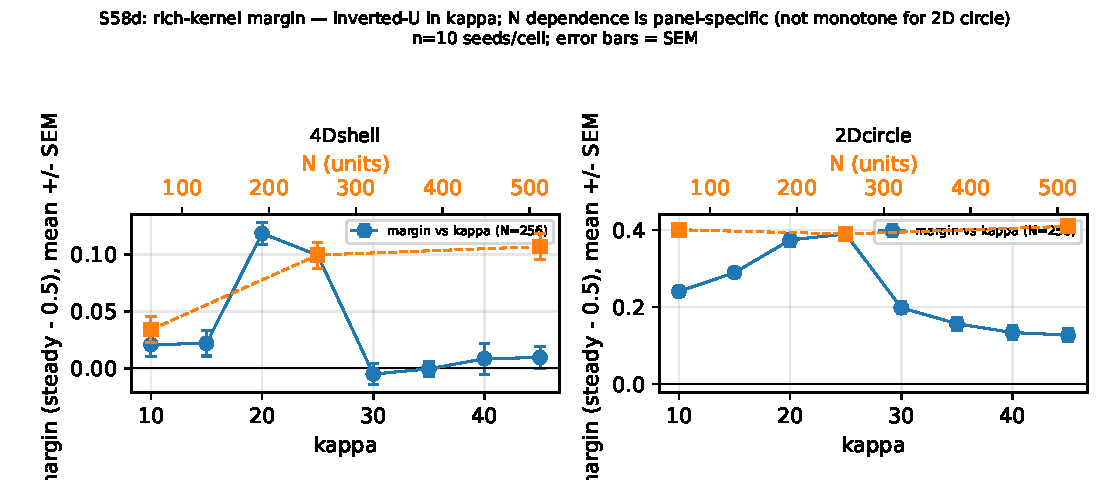
\includegraphics[width=0.95\linewidth]{self_evo_f2_margin_kappa_N.pdf}
\caption{R2: the irreducible margin on the hardest tested boundary (the
4-D shell) rises with kernel width $N$ and is an inverted-U of coupling
$\kappa$, whose sampled maximum sits at $\kappa=20$ over the eight-point grid
while the deployed $\kappa=25$ is within one seed SD of it (over-coupling
$\kappa\geq30$ collapses it); both dependences are panel-specific; the $N$
axis is flat on the 2-D circle
($0.401\to0.390\to0.410$, within seed SD) and the $\kappa$ maximum there
stays at $\kappa=25$. $n=10$ seeds per cell; error bars
are the SEM $=$ sample SD$/\sqrt{10}\approx$ SD$/3.16$, distinct from the
body's seed-level $\pm$ SD convention.}
\label{fig:margin}
\end{figure}

\begin{figure}[t]
\centering
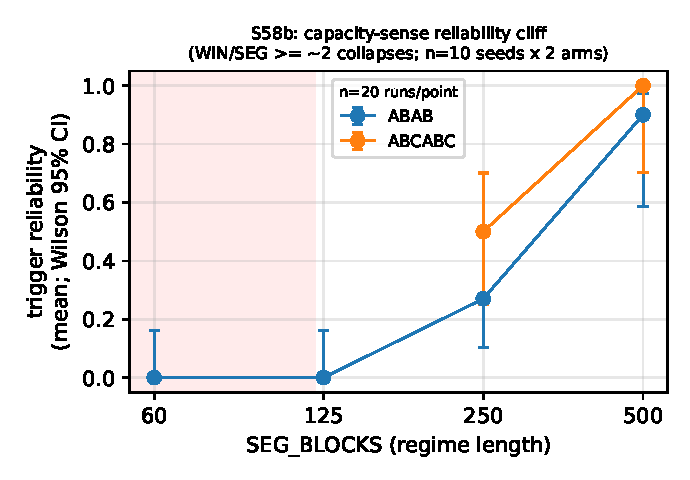
\includegraphics[width=0.62\linewidth]{self_evo_f1_reliability_cliff.pdf}
\caption{R4: reliability of the relative capacity sense degrades
monotonically with the window/segment ratio and reaches zero near ratio
$\approx2$ (shaded: SEG $\leq120$ blocks, i.e.\ ratio $\geq2$); the decline
begins well before the ratio reaches $2$, so the cliff is the approach to that
point rather than its onset. Points are means over the $10$ seeds and both
substrate arms, with
Wilson $95\%$ confidence intervals computed on the $20$ pooled runs; because
the two arms share the same capacity sense their trigger events coincide seed
by seed, so the effective sample size remains close to the $10$ seeds and the
intervals are correspondingly narrower than the evidence warrants
(Sec.~\ref{sec:r4}).}
\label{fig:cliff}
\end{figure}

\begin{figure}[t]
\centering
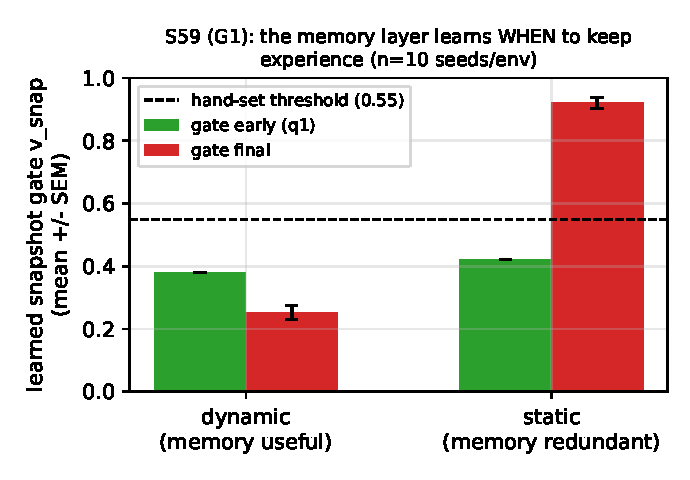
\includegraphics[width=0.62\linewidth]{self_evo_f4_vsnap_gate.pdf}
\caption{R5: the learned snapshot gate stays low when memory is useful
(dynamic) and rises when it is redundant (static); no hand-set threshold.
Bars are means over $n=10$ seeds per environment with SEM error bars
(SEM $=$ sample SD$/\sqrt{10}$); the
dashed line is the hand-set threshold $0.55$ that the learned gate
replaces.}
\label{fig:vsnap}
\end{figure}

\begin{figure}[t]
\centering
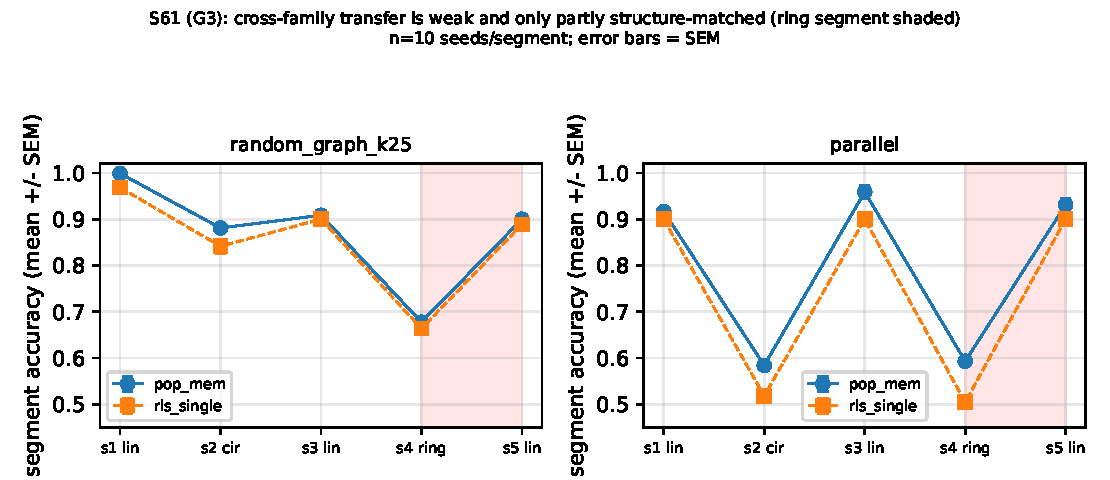
\includegraphics[width=0.95\linewidth]{self_evo_f5_cross_family.pdf}
\caption{R5: cross-family transfer is weak: the ring segment (shaded) gains
$+8.9\pm2.5$\,pp from frozen memory on the uncoupled substrate and only
$+1.4\pm1.8$\,pp on the deployed coupled one, and one family pair was tested.
Curves are means over $n=10$ seeds with SEM error bars
(SEM $=$ sample SD$/\sqrt{10}$).}
\label{fig:xfam}
\end{figure}

\begin{figure}[t]
\centering
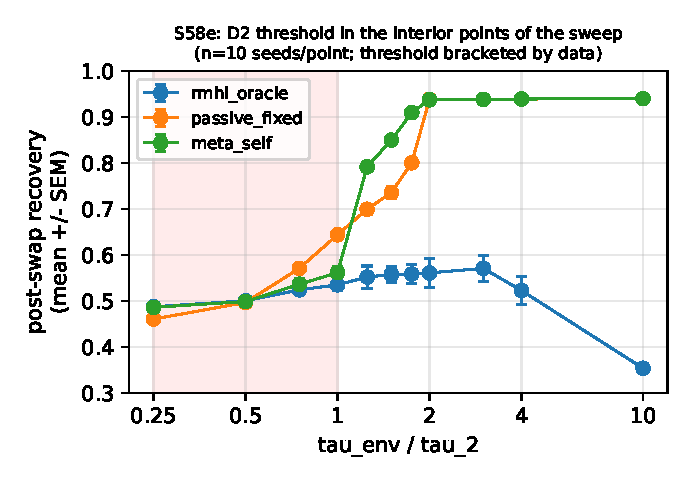
\includegraphics[width=0.62\linewidth]{self_evo_f3_d2_threshold.pdf}
\caption{R6: the D2 recovery transition band for a
reward-rate-EMA meta
layer: the post-swap accuracy stays at or near chance below the band
($0.486$--$0.561$ over the whole ratio $\leq1$ range) and recovers to
$0.94$ within it. The eleven sampled ratios include five interior points
($0.75,1.25,1.5,1.75,3$), so the transition is bracketed by measured ratios
inside $[1,2]$ rather than by its endpoints alone. The shading marks ratio
$\leq1$, where recovery fails. Curves are means over $n=10$
seeds with SEM error bars (SEM $=$ sample SD$/\sqrt{10}$; body
$\pm$ terms report sample SD).}
\label{fig:d2}
\end{figure}

\begin{figure}[t]
\centering
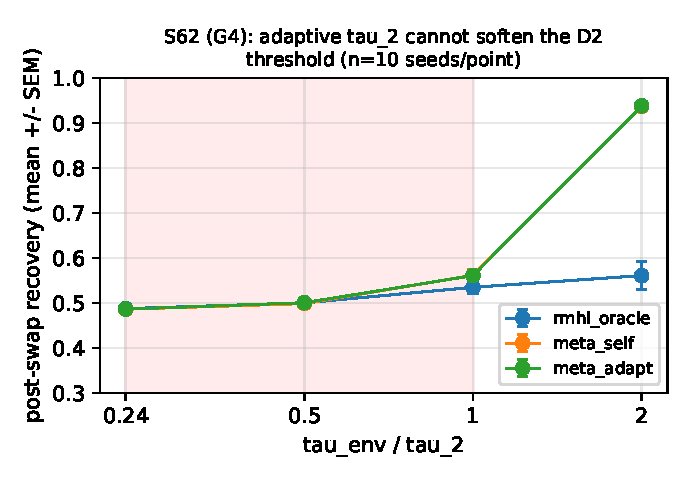
\includegraphics[width=0.62\linewidth]{self_evo_f6_meta_timescale.pdf}
\caption{R6: adapting $\tau_2$ cannot soften the D2 transition band: the
flip-plus-confirmation pipeline latency (FLIP\_CHECK $20$ + W\_EST $40$
$=60$ blocks) is the
floor. Means over $n=10$ seeds with SEM error bars
(SEM $=$ sample SD$/\sqrt{10}$); the shading marks ratio
$\leq1$.}
\label{fig:meta}
\end{figure}

\subsection{R7: content--rendering separation (supporting experiment)}
\label{sec:r7}

A natural question about
any reward-driven learner is whether \emph{the same content rendered
differently} (e.g.\ the same sentence spoken by different people, with
different tone, speed or personality) carries extra information dimensions.
s63 instantiates this on
the substrate (task generation, render construction and the complete
parameter set are given in Appendix~\ref{app:s63s64}): the semantic content
$u$ (and its fixed label $y=g(u)$) is
held identical, and a per-speaker affine render $A_s$ changes only the
physical encoding the readout observes. Two facts emerge. First, the render
is a \emph{real} extra dimension when speakers alternate (A-B-A-B, quoted at
the slowest rate, \texttt{switch\_every}$=200$ blocks; Appendix~\ref{app:s63s64}):
a single linear
readout degrades ($0.938\to0.900$, paired $t=-18.2$, $10/10$), a quadratic
expansion does not repair it ($0.889$, paired $t=-4.7$, $0/10$). The reason is
\emph{not} a geometric one: in the expanded space the readout
is not a single hyperplane, because a hyperplane in the expanded coordinates
is already a quadratic surface in the original ones. The correct reason is that the required rule is not a single function of
the observed features: the two speakers induce two \emph{different} maps from
the same physical encoding to the same label, so a correct readout must select
between two maps, and no basis built from the observed features contains the
speaker index that would let one map switch between them. Enlarging the basis
along the content coordinates therefore cannot repair the render; keeping one
hypothesis per render can, which is what the memory arm does. Frozen-hypothesis
memory with
reward-rate selection partially recovers it ($0.913$, paired $t=+9.3$,
$10/10$); the R5 memory mechanism, not the R2 capacity mechanism, is the
correct separation device.

The capacity probe \emph{registers} the
render-induced insufficiency without triggering on it, and the distinction
matters. Its held-out accuracy falls from $0.9493\pm0.0145$ in the
single-speaker condition to $0.9003\pm0.0250$ in the A-B-A-B condition
(mean $\pm$ seed SD, $n=10$; paired drop $0.049\pm0.018$, $t=8.38$, $10/10$
seeds), so the degradation is real and reproducible rather than noise. But the
largest per-seed drop is $0.084$ and the smallest $0.027$: \emph{every} seed's
drop lies below the $0.10$ relative trigger margin, so by its own criterion the
sense does not treat this as insufficiency, consistent with the deployed
setting (where the sense idles because the memory, not the readout, absorbs
the render) and with the R3 idle result, in which
$9/10$ seeds never triggered and the single trigger had no accuracy
consequence. We therefore report the probe as detecting the degradation while
staying below its trigger threshold, not as correctly flagging an
insufficiency that it then acts on: whether a $0.049$ drop should count as
insufficiency is a question about where the margin sits, not about the
measurement.

Second, the observational meta layer, i.e.\ the reward-rate-EMA controller of
Sec.~\ref{sec:r1} (scripts s40/s41/s58e), is
\emph{render-blind}: the render leaves the labels unchanged, so although
the reward rate dips transiently at each switch (hence the linear readout's
degradation), its slow EMA stays in the positive band and the meta observes
no sustained error to correct: no flip fires ($n_{\mathrm{flips}}=0$ at
every switch rate). This scopes the D2 timescale bound precisely: it governs
observing \emph{semantic flips}, not render identity; render speed is
not a hard floor for the memory mechanism's selection step, which compares
hypotheses block-by-block with no observation lag (only the snapshot
identity window of 50 blocks bounds how fast a \emph{new} render is
memorised). The same utterance is therefore not one signal but a content
dimension plus a render dimension, and the system keeps the two apart
without ever measuring the render: memory selection is purely functional:
it reads predictions and rewards, never the underlying encoding.

We state
that precisely rather than as ``no channel by construction'', which would be
too strong: the render has already altered the substrate state before any
prediction is formed, so it reaches the selection step through the predictions
the step compares. What is true is that the render is never \emph{observed}
explicitly: selection is a function of predictions and rewards, not of an
encoding label, and that is why a reward-rate selector can separate two
renders without ever being told that a render changed.

\subsection{R8: multi-source validation and the majority fallacy (supporting experiment)}
\label{sec:r8}

A second setting where a reward-driven learner can go wrong is source
conflict: when several
information sources give conflicting answers to the same content, can the
learner
find the correct one, e.g.\ by a majority (\emph{minority-submits-to-
majority}) rule. s64 instantiates this on the substrate (source construction,
drift point and the full protocol are given in
Appendix~\ref{app:s63s64}; the script and its CSV/JSON outputs are included in
the supplementary material): the same fixed
content $u$ (label $y=g(u)$) is served by five sources, each emitting a
block-level suggestion $\hat y_i$ that is either always correct
(``good'') or flips independently with probability $0.5$ (``noise'', the
hardest bad source: its reward-rate EMA sits near zero). Three facts
emerge. First, when the majority is right (3 good, 2 noise) the majority
rule works: the arms sit at the substrate ceiling, with \textit{wm} and
\textit{we} at $0.938$ and \textit{vote} and \textit{ema} at $1.000$ (the
direct-label oracle \textit{wt} is at $0.938$); the intuition holds in the
default world.

Second, when the
majority is \emph{wrong} (1 good, 4 noise) the majority rule is a fallacy:
it collapses to $0.684$, which is the analytic majority-vote value for this
configuration rather than the chance level: with one always-correct source and
four coin-flip sources, the five-source majority is right whenever at least
two of the four noise sources agree with the good one, giving
$11/16=0.6875$ (measured $0.684$). What the row shows is therefore that the
majority rule degrades to the accuracy majority voting actually delivers, and
that this value sits well \emph{above} chance; the row that reaches chance
is the all-bad one, at $0.494$. Meanwhile validation-driven selection: the
$\mathrm{argmax}$-$\bar r_{\mathrm{ema}}$ device applied to sources instead of
frozen hypotheses, keeps selecting the single good source (selection
fraction $1.000$; accuracy $1.000$ pure and $0.938$ through the worker,
bit-identical to the no-source oracle; paired $t=100.5$, $10/10$ seeds). The
learner finds the correct source by post-hoc validation, not by
counting heads.

Two features of this design bound the claim and are worth
stating with their numbers. First, what the ten seeds resample is the
substrate's time-constant realization, the content/label stream and the
per-block coin flips of the noise sources; the source reliabilities themselves
are fixed by the scenario (a good source is always right, a noise source is a
coin flip), so the contrast is close to deterministic and the paired
difference between the validation arm and the majority rule has a seed SD of
only $0.0099$. The large $t$ statistics here therefore describe a small spread
rather than a large effect: the quoted $t=100.5$ compares \texttt{ema} against
\texttt{vote}, and the same contrast routed through the worker reads $t=61.4$.
Second, on intermediate reliability: a follow-up run
(\texttt{s64b\_weak\_source\_reliability}, sources correct with
probability $0.70$, three scenarios $\times$ $10$ seeds $\times$ $2$
substrates) probes the middle where validation-based selection is
genuinely challenged. The selector still tracks reliability rather
than the crowd's opinion: in the \emph{minority-weak} scenario
(one good $0.7$ source among noise), validation-driven selection beats
the majority rule by $+0.128$ ($10/10$ seeds; worker level $+0.159$,
$10/10$) --- exactly the regime the perfect/coin-flip design could not
test. But when \emph{no} clearly-best source exists the advantage
reverses: with all sources weak, selection lands at $0.694$ vs $0.836$
for the raw vote ($0/10$), and in the majority-weak scenario the
majority rule edges validation by $+0.020$ ($1/10$ for selection).
The pattern is consistent with the mechanism: the selector's EMA
faithfully follows a $0.70$ source, so it pays the source's own error
rate, while the raw vote pools five $0.70$ sources and benefits from
their independent fluctuations; validation pays off exactly when a
reliability \emph{ordering} exists that the crowd's opinion does not
encode. The sample-complexity question (how many blocks the selection
needs at a given reliability gap) remains untested; both gaps are
listed in Limitations.

Third, the D4 boundary is reproduced for the source-consuming arms: when all
five sources are noise, every arm that consumes only source suggestions sits
at chance ($\sim0.49$) and the EMA selector finds no signal to react to
($n_{\mathrm{switches}}=242$, selection fraction $0.493$); a system whose
only input is the source set cannot recover the task, exactly as D4 states.
The \textit{wt} column of Table~\ref{tab:multisource} stays at $0.938$ in
this scenario because it is the direct-label arm: it trains on the block
label, which under the correctness channel of the main experiments is
recoverable exactly from the reward and the system's own vote (item~7 of
Appendix~\ref{app:theorems}). We therefore scope the claim: what fails when
every source is noise is not the visibility of the corruption; the
selector does register that all five candidates sit at a near-chance reward
rate, but the existence of any useful action built on the sources, and we
do not claim that poisoning is undetectable in principle.

Read column by
column, Table~\ref{tab:multisource} separates three channels rather than one
ranking: the direct-label column (\textit{wt}) is invariant at $0.938$ in
every scenario, the crowd-derived columns (\textit{vote}, \textit{wm}) follow
the majority and fail exactly where the majority is wrong
($0.684$/$0.714$) or uninformative ($0.494$/$0.492$), and the
validation-driven columns (\textit{ema}, \textit{we}) stay at the ceiling
whenever a good source exists ($1.000$/$0.938$ under a wrong majority,
$0.991$/$0.931$ under drift) while collapsing with the rest when none does
($0.494$/$0.495$). When the identity of the correct
source migrates mid-run (s64 \emph{drifting}), the majority rule stays
stuck at $0.681$ while validation re-selects the new good source
(selection fraction $0.991$, one switch, accuracy $0.991$ pure / $0.931$
through the worker; paired $t=107.4$, $10/10$); source
\emph{reliability} is tracked, not the crowd's current opinion. The two
paired $t$ values quoted for this row in the caption of
Table~\ref{tab:multisource} measure that one contrast on two different arms:
$t=107.4$ for the pure selector \textit{ema} against \textit{vote}, and
$t=57.4$ for the worker-routed arm \textit{we} against the same baseline.
The worker-routed value is the smaller of the two because \textit{we} carries
the worker's own residual error on top of the selection ($0.931$ rather than
the selector's $0.991$), which inflates the paired spread without changing
the sign or the seed count ($10/10$).

This is
the complement of the content--rendering result: there the conflict was
over \emph{render identity} with identical labels, and memory selected the
right hypothesis for the current render; here the conflict is over
\emph{labels}, and the same selection device selects the right source by
its validated history. The scope of this result is set by an explicit
assumption: validation scores each source against the block
label $y$, and we assume the selector may use that label. This is the same
information the main experiments already grant: the $\pm1$ correctness
channel determines $y$ exactly from the reward and the system's own vote
(item~7 of Appendix~\ref{app:theorems}), so s64 does not smuggle in a
hidden channel; but it does consume the label \emph{directly and per
source} rather than only through the system's own vote, and its results are
therefore conditional on that reading and are not evidence for R1--R6,
whose claims are made without ever forming $y$.

Two consequences follow.
First, the direct-label arm (\textit{wt}) is not privileged beyond what
item~7 already allows, so the comparison s64 actually makes is between
source-based channels and direct label use, not between a system with and
without labels. Second, if the feedback were aggregated across sources or
delayed by more than one block, the selector would degenerate to the
majority rule it was meant to outperform, and with no good source at all it
cannot repair the situation (D4).

\begin{table}[t]
\centering
\footnotesize
\caption{Multi-source validation (supporting experiment R8): mean accuracy by
scenario on \textit{random\_graph\_k25} (5 sources, $K{=}20$, $T{=}40000$,
$n=10$ seeds).
\textit{wt} is the no-source oracle (trains on the true label);
\textit{vote} is the majority rule over the five suggestions;
\textit{wm} trains on the majority suggestion; \textit{ema} emits the
suggestion of the highest-reward-rate-EMA source; \textit{we} trains on
that source (the same reward-rate-EMA $\arg\max$ selection device that R5
applies to frozen hypotheses, applied here to sources). Paired $t$ vs
\textit{vote} on the
minority-good row: $t{=}100.5$, $10/10$; on the drifting row: $t{=}107.4$
(ema) and $t{=}57.4$ (we), $10/10$.}
\label{tab:multisource}
\begin{tabular}{@{}lccccc@{}}
\toprule
Scenario (good+noise) & \textit{wt} & \textit{vote} &
\textit{wm} & \textit{ema} & \textit{we} \\
\midrule
majority-good (3+2) & 0.938 & 1.000 & 0.938 & 1.000 & 0.938 \\
minority-good (1+4) & 0.938 & \textbf{0.684} & 0.714 & \textbf{1.000} & \textbf{0.938} \\
all-good (5+0) & 0.938 & 1.000 & 0.938 & 1.000 & 0.938 \\
all-bad (0+5) & 0.938 & 0.494 & 0.492 & 0.494 & 0.495 \\
drifting (migrates) & 0.938 & \textbf{0.681} & 0.715 & \textbf{0.991} & \textbf{0.931} \\
\bottomrule
\end{tabular}
\end{table}

\section{Discussion}
\label{sec:disc}

\paragraph{Positioning.} The contribution is the \emph{autonomous}
correction stack on a standard error-driven base: the capacity sense that
decides when and to what to expand, the memory that preserves solutions and
masks readout divergence (Sec.~\ref{sec:r5}), the multi-level chain (which
expands twice and then stops at its ladder cap, leaving the ring
unrepresented; Sec.~\ref{sec:r3}), and the verified timescale band
(Sec.~\ref{sec:r6}). We note plainly
that a plain error-driven learner matches the single-task performance of
the full stack; the value is in the autonomous, hierarchical,
self-monitoring structure, and in the negative results that bound it.

Each component is a standard technique and we name it as such rather than
presenting it as a new mechanism: the direction detector is sign detection
on a slow reward-rate EMA with a tracked flip magnitude (a two-armed
decision rule), the memory selector is an argmax over exponentially weighted
reward estimates, the capacity sense is a ridge (and PCA-ridge) probe
thresholded on a validation statistic, the basis ladder is a zero-padded
polynomial feature expansion, and the snapshot gate is value learning
applied to a retention decision. What is studied here is how those pieces
compose under one correctness-only channel, where each of them stops
working, and what boundaries follow. We also state the limits of that
comparison: our one external competitor is EWC \cite{kirkpatrick2017}, run
under the same protocol at a matched optimiser (R3); we did not run a
reservoir-specific online-learning method, and we run no supervised baseline
at matched budget, so nothing here should be read as a claim about the
relative accuracy of this stack against published methods beyond that single
contrast.

The distinction from supervised learning is therefore not accuracy but
\emph{autonomy at the decision level}: a readout that is handed the label
every step matches (and often beats) the stack on single-task accuracy, but
it learns nothing about \emph{whether} or \emph{how} to correct itself, and
it cannot keep, reuse, or bound experience. The stack earns its keep not by
being more accurate but by discovering, repairing, and reusing under a
correctness-only channel that, as item~7 makes explicit, carries the
same information as a one-step-delayed label, and by knowing, from its own
observation scale and pipeline floor, when it cannot act (R4, R6). This complements, rather than competes with,
reservoir-computing practice
\cite{lukosevicius2009,tanaka2019}, consolidation-based memory models
\cite{fusi2005,benna2016}, and continual-learning architectures
\cite{parisi2019,kirkpatrick2017}.

\paragraph{Autonomy versus self: a formal distinction.}
``Autonomy at the decision level'' is a claim about \emph{where the policy
lives}, not about accuracy and not about a phenomenal subject. Formally, the
environment supplies a correctness channel $r_t\in\{-1,+1\}$ and never an
action $a_t$; the system supplies the map from its own history to a decision
(flip or not, freeze or not, expand or not, which hypothesis to read out).
Autonomy is therefore endogeneity of that map at decision time: the
environment scores the system, it does not drive it. The paper claims this
and nothing stronger; the $\pm1$ channel is still an environment-supplied
feedback budget, and item~7 of Appendix~\ref{app:theorems} makes explicit
that it is informationally equivalent to a one-step-delayed label.

``Self'' is used here in an operational, not a metaphysical, sense. A minimal
self in this stack is a triple of properties of the system's own internal
state $S$: (i) \emph{persistence}---$S$ survives regime revisits rather than
being rebuilt from the environment each block; (ii) \emph{functional
identity}---components of $S$ are named by what they predict, not by an
external identifier (R5's prediction-agreement key, not a geometric
fingerprint); and (iii) \emph{causal use}---$S$ is an input to subsequent
decisions rather than a logged afterthought. Under that definition the four
mechanisms already reported are the stack's self-seeds, and they are not
interchangeable:

\begin{itemize}[leftmargin=1.4em,itemsep=2pt,topsep=2pt]
\item \emph{Agency} (R1): the reward-rate sign is a read of ``my last
direction was wrong,'' from a statistic the system itself aggregates. The
discrete flip $w\to-w$ is an act, not a fitted parameter update.
\item \emph{Growth} (R3): the relative capacity sense attributes
``representation insufficient'' to the feature map when a richer nested
basis recovers what the current one cannot, and refuses the rung when it
does not (ring, ladder cap).
\item \emph{Memory} (R5): frozen snapshots are persistent, functionally
identified experience; selection among them is the reuse of one's own past
solution rather than re-adaptation from scratch.
\item \emph{Temporal self-model} (R6): the flip-plus-confirmation pipeline
latency ($60$ blocks; detection component FLIP\_CHECK $=20$, measured
detection latency $39$) is a measured lower bound on the timescale of one
\emph{confirmed} action of the meta operator. Knowing that one cannot act
faster than one's estimator is a
self-bound, not a property of the task.
\end{itemize}

Without (i)--(iii) the same mechanisms are reactive control. With them the
stack has a decision-level self and decision-level autonomy at once, and the
two must not be collapsed: a label-fed readout can be accurate and still have
no self of this kind (nothing it keeps is its own), while this stack can have
a self of this kind and still match---rather than beat---that readout on
single-task accuracy. We claim the latter conjunction and not the former
advantage.

\paragraph{Self-attribution, self-verification, self-bounding.}
Self-attribution is the map the stack already implements from its observables
to a failure-cause class. Its domain is the closed set the system can
actually see: the reward-rate EMA $\bar r$ (and its post-flip change
$\Delta\bar r$), the relative capacity-probe score and its hold pattern, the
pipeline latency, and the selected hypothesis's own reward rate. Its range
is the finite class the mechanisms distinguish, not an open causal model of
the world. Writing $O=(\bar r,\Delta\bar r,\text{probe-}\delta,\text{hold},
\text{latency},\bar r_{\mathrm{sel}})$ for that observation tuple, the
implemented attribution map is
\[
A:\;O\;\longmapsto\;\{\text{direction},\ \text{representation},\
\text{memory},\ \text{timescale},\ \text{none}\},
\]
where the four non-residual classes abbreviate direction error,
representation insufficiency, memory miss, and timescale mismatch.
A collapse of $\bar r$ that a candidate flip is estimated to reverse
attributes \emph{direction error} and licenses the R1 operator. A held probe
deficit against the current basis attributes \emph{representation
insufficiency} and licenses R3 expansion (or, on the deployed substrate,
idles, because the deficit does not appear). A revisit whose frozen
hypotheses carry higher $\bar r$ than the continuously adapted worker
attributes \emph{memory miss} to ``we have solved this and discarded it,''
which is what R5's selector acts on. An environment change faster than the
estimator's bandwidth attributes \emph{timescale mismatch}, not ``no
direction exists'' (R6, D2). ``None'' is the residual class and is taken when
no intervention is triggered.

Self-verification is the closed loop that turns each attribution into a
test: flip and re-measure $\Delta\bar r$ (D1); expand and re-sense; select a
frozen hypothesis and observe whether its reward rate holds. Attributions
are therefore not beliefs about the environment; they are action-conditioned
readings of the system's own statistics, and they are only as good as the
operator that consumes them. Two boundaries of that map are already
measured. First, \emph{signal corruption is not in the range}: a polluted
reward that is still informative enough to drive $\bar r$ produces the
attribution ``none'' while accuracy collapses (s42, D4); the same channel
cannot certify its own trustworthiness. Second, \emph{weight-norm blow-up is
not in the domain}: the worker's RLS covariance wind-up is visible to a
researcher with access to $w$, and is invisible to a stack whose observables
are the quantities above; the memory layer masks the \emph{consequence} of
that divergence without ever attributing it (s58c, R5). We do not claim a
complete diagnosis, only the finite partition the deployed mechanisms
instantiate.

Self-bounding is the dual of attribution: knowing when \emph{not} to act.
R4's reliability cliff is a self-bound on expansion (a held probe deficit
that the window/segment ratio cannot certify is not a license to expand);
R6's pipeline floor is a self-bound on the meta operator (no \emph{confirmed}
flip cadence
faster than $60$ blocks, detection alone every $20$); the ladder cap is an open self-bound (no rung left
to refuse). Taken together these three are the sense in which the stack
``knows when it cannot act'': not as an introspective report, but as a set
of measured abstentions.

\paragraph{Negative results: self-repair (s58c) and self-verification (s42).}
Two of the boundaries above are controlled negative results and are cited as
such; a third item that once looked like one is not, and is treated in the
next paragraph. The three must not be mixed.

\emph{Memory does not prevent divergence; it masks its consequence}
(s58c, R5). Both arms of the multi-level experiment measure weight norm and
accuracy: a memoryless RLS worker chasing an unfittable ring boundary
diverges to weight norm $\sim2800$ (max $3265$) and collapses to chance
($0.504$), while the frozen-snapshot selection arm reaches $0.801$ under an
\emph{identical} worker divergence. What changes is which hypothesis is read
out, not whether the worker blows up. This is a negative result about the
repair mechanism itself (self-repair via memory is selection under
divergence, not prevention of it), and it is the reason R5 is phrased as
masking rather than protection.

\emph{A polluted reward drives self-deception and cannot be self-detected}
(s42, D4, item~5 of Appendix~\ref{app:theorems}). In a controlled
corruption of the correctness channel over blocks $1200$--$1700$ of $2000$,
accuracy inside the window falls to $0.106\pm0.014$ (uncoupled) and
$0.064\pm0.008$ (coupled), and the meta layer flips \emph{more} often
($3.0$ versus $1.0$ in the uncorrupted control) without either arm's
post-window accuracy separating. This is a negative result about
self-verification: the stack optimizes the signal it measures, and the
signal cannot vouch for itself. It is also why self-attribution's range,
stated above, excludes ``corrupted reward'' as an output class.

\paragraph{Why no per-dimension gain operator is claimed.}
\begin{sloppypar}
A per-dimension structural gain is \emph{not} claimed, and the boundary is
worth stating precisely because it is easy to over-read. The dedicated
isolation arm (\texttt{s47\_self\_correction\_gain}) was run at script level
against the archived data ($10$ seeds); its pre-registered self-correction
prediction (P2: a reward-driven scalar boost improves the R2/R3 shift
regimes without costing R1/R4) is marked \texttt{[REFUTED by own data]} in
the script header, and its adaptivity prediction (P3) is marked
\texttt{[NOT VERIFIABLE]} because the boosted arm saturates at the high-$\eta$
control. No number from that arm is cited in this manuscript: the arm is a
withdrawn design attempt, not a measurement of the field. What the paper
retains is weaker and positive: the only correction the stack demonstrates
is the uniform sign flip $w\to-w$, which is not a per-dimension gain; the
operative design criterion is whether an operator's magnitude scales with the
noisy reward in the $\mathbb E[r]\approx0$ dead zone (a positive-feedback
trap), not whether its gain is per-dimension. The correct reading of s47 is
therefore ``its own pre-declared prediction failed; its numbers are not
adopted''---not ``a negative result about structural correction.''
\end{sloppypar}

\paragraph{Hosts and portability.}
The mechanism stack reported here is demonstrated on one host: the
recurrent relaxation reservoir of Methods (a readout-level stack on
$257$--$769$ block-mean features). Companion work on the REDEM-SSM host
(Diagonal state-space model) occupies a different layer of the same program
(readout form and metric, not decision-layer autonomy), and the decision-layer
mechanisms studied here are not transferred onto that host in this paper. A
design study of that port (referred to elsewhere in the program as G) is
explicitly \emph{not} part of the present manuscript: porting a
substrate-agnostic decision stack onto a host whose feedback budget is
richer (per-token labels rather than $\pm1$) is a re-run with a different
autonomy ceiling, not a contribution of this paper. The claim of this paper
is therefore host-scoped: decision-level autonomy and a minimal operational
self, on this substrate, under this feedback budget.

\paragraph{Methodological notes.} Four corrections shaped the picture, and we
report them rather than leaving them implicit.
\begin{itemize}[leftmargin=1.4em,itemsep=2pt,topsep=2pt]
\item Capacity probes on high-dimensional block-mean features must be
well-conditioned. A full-dimension ridge misreads true capacity, which is why
the original ``circle undecodable'' claim was an artifact.
\item At $\dim\geq4$ label balance forces the balanced ball to clip the unit
cube, which breaks dimension as a monotone stress axis.
\item The complexity axis leaves an irreducible margin: even six quadratic
surfaces leave an irreducible $\sim+4$--$6$\,pp edge, and the trend across
complexity is flat-to-rising rather than degrading.
\item The capacity sense's reliability cliff is structural. It is unfixable by
its margin, by its window, or by a self-adapted observation scale, and
exposure count is the only repair the archived runs demonstrate.
\end{itemize}

\paragraph{Limitations.} The demonstration is a CPU numerical study of one
physics-inspired substrate model and one protocol family; no device was
fabricated and no measurement is reported, so nothing here is evidence about
hardware behaviour, and the ``adaptive experience system'' is established in
this setting, not as a universal theorem. Three scope conditions follow from
the design of the study and bound every autonomy and self claim above.
First, \emph{a single substrate}: all decision-layer results are on the
recurrent relaxation reservoir of Methods; the REDEM-SSM host of the
companion line is not an alternative host for these mechanisms here, and a
port of the stack onto that host is a separate design program, not a result
of this paper. Second, \emph{a single feedback budget}: every autonomy claim
is made under the $\pm1$ correctness channel alone (plus whatever that
channel determines through the system's own vote, item~7); richer feedback
(per-token labels, dense rewards) is a different regime in which the reasons
for most of these mechanisms disappear, and we run no matched comparison
against such a regime. Third, \emph{no embodied closed loop}: the system
acts only through a readout weight and a finite decision set (flip, freeze,
select, expand); there is no sensorimotor cycle, no environment whose
dynamics the system's actions change beyond the prescribed protocol events,
and no body whose failure modes could ground the operational self defined
above outside the numerical stream. The operational self is therefore a
property of this decision stack under this protocol, not evidence about
organisms or about a physical device. The structural-correction
criterion is explicitly \emph{not} a demonstrated per-dimension mechanism:
the only operator the stack applies is a uniform sign flip, and the
dedicated gain-modulation arm (\texttt{s47}) is not used as evidence:
its pre-declared prediction is not supported by its archived data and
its numbers are not adopted here (see Discussion). Several claims are bounded by the
range actually tested rather than by an argument: the absence of collapse on
the coupled substrate holds for the boundary families tried (up to six
quadratic surfaces), the ring's non-expansion holds for the nested basis
ladder tried (linear through cubic coordinate powers), and the coupling
$\kappa=25$ is a model choice supported by an eight-point sweep, so the
capacity peak is located only to $\kappa\approx20$--$25$ on the tested grid
and the deployed value is not presented as that peak.

The
reliability figures of R4 are rates over autocorrelated per-window decisions
and are therefore trend-level rather than sharp, and their product form
assumes, without verifying, that the two factors are independent. The
paired comparisons reported throughout are exploratory in the
multiplicity sense: they are per-claim paired tests and sign counts at
$n=10$ seeds, with no family-wise error-rate or false-discovery-rate
correction applied across the paper's comparisons, and the $k/n$ sign counts
are descriptive summaries rather than tested statistics. A
substantial set of constants is hand-set rather than learned: the
memory/selection thresholds that remain hand-set are architectural
(capacity, agreement window), while the snapshot gate itself is now learned.

Cross-family transfer is weak, rests on a single family pair, and is absent on
the deployed coupled substrate. The external comparison is one method deep:
EWC \cite{kirkpatrick2017} is run at a matched optimiser and does not improve
the revisit run, but no reservoir-specific online-learning method and no
supervised baseline at matched budget is compared,
and the stack matches rather than exceeds a label-fed readout on single
tasks. The D2 recovery transition band is
pipeline-bound (FLIP\_CHECK $+$ W\_EST $=60$ blocks, flip-plus-confirmation);
whether any
adaptation of the observation scale could lower it was not measured
(no open-loop $\tau_2$ scan), and ``faster observation costs decision
noise'' is not offered as a measured trade-off. The transition itself is
located only to the interval $[1,2]$ in which the added interior ratios
bracket it, not to a point.

Three gaps follow from decisions that were not
taken rather than from results that came out badly, and we list them so they
are not read as measurements. No fixed-protocol scan over the meta's
observation scale $\tau_2$ was run: what exists is a closed-loop controller
whose rate is bounded to $\tau_2\in[5,50]$ blocks; no open-loop $\tau_2$
scan exists, so no decision-noise trade-off is claimed. The
multi-source experiment's sources are fixed at $1.0$ or $0.5$ in the
archived run (seed spread correspondingly tiny, $0.0099$), so its
equivalence-class results are precise but narrow; an
intermediate-reliability follow-up (\texttt{s64b}, sources at $0.70$)
is summarized in R8 and locates where validation selection pays
(majority-weak ordering: $10/10$) and where it does not (all-weak:
$0/10$), but no sample-complexity curve over reliability gaps or block
budgets was run. And no
higher basis rung exists above the cubic one, so the ring refusal observed at
the top of the ladder cannot be separated from a shortage of rungs.

\section{Conclusion}
\label{sec:concl}

In CPU numerical simulation, on a recurrent relaxation reservoir under
$\pm1$ reward, we established that an autonomous correction stack is
feasible. Its parts are direction
detection and structural correction (R1); a well-conditioned capacity sense
and the corrected representation-sufficiency picture (R2); the composing
self-evolution loop (R3); the sense's bounded but exposure-rescuable
reliability (R4); and a memory layer that identifies, protects, self-tunes and
transfers only weakly and not on the deployed substrate (R5). The last part is
a measured
meta timescale bound that is a bandwidth property of the estimator rather than
a theorem about the system (R6). Two supporting experiments are reported in
Results: content--render separation (R7) and multi-source validation with the
majority fallacy (R8); both are reported as supporting experiments, and the
multi-source result is conditional on consuming the block label per source
and is not evidence for R1--R6 (Sec.~\ref{sec:r8}).

Two qualifications bound what that means. First, the stack confers no
single-task accuracy advantage: a supervised readout fed the label at each
step matches it, and the one external competitor we run (EWC, R3) does not
improve the revisit run either, so the memory gain is measured against
continuous re-adaptation and that baseline rather than claimed as general
superiority. Second, the demonstrated autonomy is at the decision level
only and is partial in practice. The thresholds on which triggering and
correction rest (coupling, block size, reward-rate timescale, probe window,
trigger margin, hold requirement, cooldown, slot capacity, forgetting
factor) remain architectural constants, and only the snapshot gate is
adapted by a fixed-step rule (two hand-set hyper-parameters). The
operational self defined in Discussion---persistence, functional identity,
causal use---is therefore a decision-stack property on one substrate under
one feedback budget, with no embodied closed loop and no claim of a
phenomenal subject; self-attribution is the finite partition those
mechanisms instantiate, not an open causal model, and its range excludes
both corrupted reward (s42) and unobserved worker divergence (s58c).

Within those limits the
system accumulates, retains and reuses experience without manual
intervention at the decision level, adapts its snapshot threshold by a
fixed-step rule with two hand-set hyper-parameters, and
knows, from its own observation scale and the pipeline floor, when it
cannot act. The failure boundaries are part of the result rather than
exceptions to it. The expansion mechanism is demonstrated only on the
uncoupled testbed and idles on the deployed substrate. The multi-level chain
reaches its top rung on $5/10$ seeds and leaves the ring unrepresented, an
open failure at the ladder's cap rather than a refusal we can certify. The
reliability of the capacity sense degrades monotonically with the
window/segment ratio ($0.90$ at ratio $\approx0.48\to0.27$ at
$\approx0.96\to0$ near ratio $\approx2$) and is unrepairable by its own
margin or window; only exposure count helps. The memory layer's advantage is partial, and
its cross-family transfer is weak and absent on the deployed substrate. And
the meta layer cannot correct changes much faster than its own observation
scale.

\section*{Declaration of competing interest}
The author declares no competing interests.

\section*{Funding}
This research did not receive any specific grant from funding agencies in
the public, commercial, or not-for-profit sectors.

\section*{Data availability}
\begin{sloppypar}
The simulation scripts for this paper (the \texttt{s39}--\texttt{s65}
series listed in Appendix~\ref{app:index}), the frozen dependency set they
import (\texttt{paper\_e/deps/}), the six figure PDFs, and the archived
CSV/JSON result files that back the numbers reported here are provided as
Supplementary Material accompanying this submission
(\texttt{Supplementary\_Material\_PaperE.zip}). Three scope notes keep this
statement checkable. First, the multi-source validation experiment of
Sec.~\ref{sec:r8} is inside that archive in the same form as every other
experiment reported here: the script \texttt{s64\_multi\_source\_validation.py}
and its result files are present under \texttt{scripts/} and \texttt{data/}, so
this work does not depend on material that has to be requested separately.
Second, the public REDEM repository \cite{redemrepo}
hosts the earlier companion
projects (\texttt{paper\_a}--\texttt{paper\_d}) and their shared simulator
dependencies; the \texttt{paper\_e} material listed above, including every
script and result behind the numbers reported here, is delivered in the
supplementary archive named above. The companion
manuscripts carry Zenodo \emph{concept} DOIs (all-versions, always-latest;
not a single-version DOI), namely
(\url{https://doi.org/10.5281/zenodo.22109664},
\url{https://doi.org/10.5281/zenodo.22110606},
\url{https://doi.org/10.5281/zenodo.22110618},
\url{https://doi.org/10.5281/zenodo.22110623} for companions A, B, C and D
\cite{companionA,companionB,companionC,companionD}). Third, the boundary between
this paper and that companion series is drawn explicitly: the physical
substrate and its phase diagram belong to companion A, the online-learning
architecture belongs to companion B, and the mechanism dissection belongs to
companion C. This paper's contribution is the correctness-only self-evolution
stack built on that substrate (the capacity sense, the frozen-hypothesis memory
layer, the multi-level chain and the meta-timescale bound), and the three
companions are cited here as premises rather than restated, so the results
reported here are not evidence for theirs and theirs are not evidence for
these.
\end{sloppypar}

Finally, and in the same
spirit, what this archive does and does not contain is stated literally, so
that the reproducibility claims can be checked rather than assumed. It does contain: every script of the
\texttt{s39}--\texttt{s65} series as source, the frozen dependency modules they
import, the six figure PDFs and the archived CSV/JSON pairs; each CSV row
records its run's seed index (\texttt{seed\_idx}) and each JSON records the
constant block of that experiment (including the substrate topology seed), so
the ten seeds can be identified and re-run individually. It does not contain:
a commit hash or release tag (the material is delivered as this archive rather
than from a versioned public repository; the public repository
\url{https://github.com/huyamingc/REDEM} carries an MIT LICENSE and a
\texttt{requirements-lock.txt} pinning the interpreter-side package versions
used for the archived runs, and this archive is a snapshot of that state), a lock file or interpreter and
package version pins (the dependency set is frozen as source in
\texttt{paper\_e/deps/}, and no Python/NumPy version strings are written into
the archived JSON; the repository-level lock file named above covers this
gap), or an explicit license inside the archive, which is attached at the
repository level (MIT) and will accompany the deposited version.

\section*{CRediT authorship contribution statement}
\textbf{Yaming Hu}: Conceptualization, Methodology, Software, Validation,
Formal analysis, Investigation, Data curation, Writing -- original draft,
Writing -- review \& editing, Visualization. The CRediT roles not listed
here (Funding acquisition, Resources, Supervision, Project administration) do
not apply to this single-author, self-funded study.

\section*{Declaration of generative AI and AI-assisted technologies in the
writing process}
During the preparation of this work the author used an AI-assisted
writing and review tool in order to improve readability, check consistency
and draft editorial text. After using this tool, the author reviewed and
edited the content as needed and takes full responsibility for the content of
the publication.

\section*{Acknowledgements}
The author thanks the open-source community whose tools supported this
research.

\appendix

\setcounter{table}{0}
\renewcommand{\thetable}{A\arabic{table}}

\section{Findings and empirical claims index}
\label{app:theorems}

This index collects the twenty-four statements the paper relies on and
classifies each by the kind of support it actually has, rather than naming
them all theorems. The label at the head of each item is that
classification: \emph{Theorem (analytical)} for a statement proved from the
stated model assumptions; \emph{Proposition (analytical, checked
numerically)} for a short analytical consequence that is also tested against
the archived runs; \emph{Proposition (analytical, blockwise-conditional)}
for an identity that holds block-by-block under a stated condition on the
block statistic, with the condition's coverage stated inside the item;
\emph{Empirical finding} for a measured regularity of
this substrate and protocol; \emph{Empirical finding (scoped)} where the claim
is bounded to the range actually tested; \emph{Design criterion} for a
modelling rule that is motivated rather than proved; and \emph{Conjecture}
for an open statement. The parenthetical source at the end of each item
(R1--R8) names the Results subsection that carries the evidence, whose scripts
and archived data files are listed in Appendix~\ref{app:index}; where a
statement is empirical, the conditions under which it was measured
(substrate, tested range and sample size) are stated inside the item.

\begin{enumerate}[label=\arabic*.]
\item \emph{Proposition (analytical, blockwise-conditional).} \textbf{Mirror impossibility.} Under the protocol's block vote
$\mathrm{vote}=\mathbb 1[\bar o>0.5]$ (Methods) with an unbiased linear
readout and a fixed block size $K$, negating the readout weight negates the
block mean, $\bar o\mapsto-\bar o$. On a block where $|\bar o|>0.5$ this
gives $\mathrm{vote}(-w)=\mathbb 1[\bar o<-0.5]=1-\mathrm{vote}(w)$ and
hence $r(-w)=-r(w)$ blockwise. The identity is blockwise-conditional, not
global: on the dead zone $|\bar o|\le 0.5$ (which contains the tie set
$\bar o=0.5$ but is strictly larger for this readout family, since a linear
readout with $W_0=\mathbf 0$ initialization routinely produces block means
inside it) both arms emit class $0$, so $\mathrm{vote}(-w)=\mathrm{vote}(w)$
there and the two arms \emph{agree} rather than mirror; the deterministic
tie rule at $\bar o=0.5$ (both classes $0$; $K=20$ is even, so the exception
is stated here rather than excluded by an odd-$K$ assumption) is the
measure-zero boundary of that dead zone. The fraction
$P(|\bar o|\le 0.5)$ of dead-zone blocks is a property of the readout's
converged state distribution, is not fixed by the protocol, and is not
derived here; the archived R1 runs operate far from it (the mirror
hypothesis is wrong on essentially every post-inversion block, Methods), so
the blockwise identity carries the R1 argument on those runs. If in addition
the state distribution is taken to be independent of $w$ (a deterministic
mirror assumption, assumed here rather than derived), then
$\mathbb E[r](-w)=-\mathbb E[r](w)$ on the non-dead-zone blocks, and no
suppression is learnable inside the
two-arm mirror set by \emph{RMHL-type local reward-driven rules}. The
global discrete flip of the meta-layer is an outside-of-the-mirror-set
operation (it exploits, rather than learns, the mirror symmetry) and is
therefore not covered by this bound (R1).
\item \emph{Proposition (analytical, checked numerically).} \textbf{D1 sign-ambiguity dissolution.} Each meta-level learns from the
reward-rate change $\Delta r$ (the EMA-level difference after a flip),
which is convention-free in the sense that a sign flip of the reward
convention maps $\Delta r\mapsto-\Delta r$ and the flip decision is
equivariant under it (R1).
\item \emph{Empirical finding (scoped)}. \textbf{D2: tracking-bandwidth limit of the meta estimator.} For a
reward-rate-EMA meta layer, a system can only correct
changes slower than its observation scale, because a first-order low-pass
estimate cannot follow a change faster than its own time constant
\cite{haykin2002}; the statement is a bandwidth property of the estimator
rather than a theorem about the system, and the measured form for this stack is
a monotone
recovery transition band at
$\tau_{\mathrm{env}}/\tau_2\approx1$--$2$ (empirical, this substrate, sampled
at eleven ratios with five of them inside $[1,2]$, so the band is bracketed by
measured points),
quantitatively $\tau_{\mathrm{env}}\gtrsim$ the flip-plus-confirmation pipeline latency of $60$
blocks $=1.2\,\tau_2$, which is the same constraint (R6).
\item \emph{Conjecture}. \textbf{D3 regression boundary.} Finite hierarchy plus
fixed top-level rule; infinite bootstrapping would violate the
self-reference boundary. Stated as an open conjecture, not a proven
theorem (theory).
\item \emph{Empirical finding}. \textbf{D4 signal trust.} A self-evolving system optimizes the signal
it measures; a polluted signal drives self-deception and cannot be
self-detected (R1).
\item \emph{Proposition (analytical, checked numerically).} \textbf{1-D completeness.} Mirror-flip is complete for
inversion-class regimes, while translation/compression regimes collapse
(R1).
\item \emph{Theorem (analytical).} \textbf{$\pm1$=label identity.} $r=+1\Rightarrow y=\mathrm{vote}$,
$r=-1\Rightarrow y=1-\mathrm{vote}$, both exact. Consequence: the
correctness-only channel is informationally equivalent to a one-step-delayed
label: the label is not transmitted, but it is fully determined by the
reward and the system's own vote, so any consumer of this channel is
label-informed, and results obtained under it are not evidence of
label-free learning (R1, Methods).
\item \emph{Proposition (analytical, checked numerically).} \textbf{Rule-selection criterion.} Credit-assignment failure is rule
selection, not an information-theoretic limit (R1).
\item \emph{Design criterion}. \textbf{Structural-correction criterion.} In the
regimes studied here, a correction operator whose magnitude scales with the
noisy reward signal (a scalar gain acting in the $\mathbb E[r]\approx0$
dead zone) is a positive-feedback trap and a noise amplifier (R1). The
criterion is therefore about whether the operator scales with that signal,
not about per-dimension gain as such: the only correction the stack
demonstrates is the uniform sign flip $w\to-w$, a single scalar sign change
applied to all weight coordinates together, which is not a per-dimension
gain. The criterion is reported as a design motivation supported by that
observation, not as a proved necessity.
\item \emph{Empirical finding}. \textbf{L2 decodability.} Smooth rotation is linearly decodable from
the coupled substrate and trackable online; speed is absorbed (R2).
\item \emph{Design criterion}. \textbf{Probe-conditioning criterion.} Capacity probes on high-dim
block-mean features must be well-conditioned (R2, methods). The raw-feature
capacity figures quoted in R2 and in Table~\ref{app:numbers}
($0.84\pm0.06$ for the coupled substrate, $0.55\pm0.05$ for the uncoupled one; here the $\pm$ is the population SD over the pooled readings)
are read directly from the \texttt{raw\_capacity\_probe} field of
\texttt{data/s53\_auto\_basis\_v1.json} (top-$50$ PCA ridge on raw block-mean
features, $240$-block windows refitted every $20$ blocks, $\lambda=1.0$,
$n=2550$ readings per substrate over $10$ seeds and three arms), which closes
the traceability gap between that number and the script that produces it.
\item \emph{Empirical finding}. \textbf{L3 = boundary complexity, not dimension.} The ball degrades
2-D$\to$3-D but 4-D balance clipping breaks the dimension axis; the annulus
declines with dimension (R2).
\item \emph{Empirical finding (scoped)}. \textbf{L3: no collapse in the tested range.}
Within the boundary families tested (up to six quadratic surfaces),
accuracy stays above chance and no collapse is observed; over the same range
the measured trend in complexity is flat-to-slightly-rising ($0.544\pm0.010$
to $0.559\pm0.015$ from two to six quadratic surfaces), so the finding is the
absence of a complexity-driven collapse rather than a degradation that has
levelled off, and ``saturation'' is not used as a synonym for it. Full collapse
was obtained only on the uncoupled substrate. Since a linear readout on a
fixed feature space has capacity bounded by the feature count, this is
reported as a bounded empirical finding over the tested range rather than as
a universal no-collapse theorem (R2).
\item \emph{Empirical finding (scoped)}. \textbf{Rich-kernel saturation (corrected).} The irreducible margin
rises with kernel width on the hardest tested boundary (flat beyond
$N=256$, and flat over all three widths on the $2$-D circle, both within seed
SD) and is
inverted-U in coupling over the eight-point grid
$\kappa\in\{10,15,20,25,30,35,40,45\}$: the sampled maximum lies at
$\kappa=20$ ($0.1185\pm0.031$) with the deployed $\kappa=25$
($0.0995\pm0.036$) within one seed SD of it, the margin collapses at
$\kappa\geq30$, and on the $2$-D circle the maximum stays at $\kappa=25$;
the deployed value is therefore \emph{not} presented as the capacity peak and
no optimal coupling is claimed (R2).
\item \emph{Empirical finding}. \textbf{L4 dynamic memory.} Frozen hypothesis memory + reward-rate
selection beats continuous re-adaptation under revisits ($+5.0\pm0.9$\,pp
overall, $+14.9\pm4.1$\,pp on the circle revisit; the per-segment gains are
$+4.2$, $+3.6$, $+2.6$ and $+14.9$\,pp, of which only the linear-revisit gain
fails to reach the $5\%$ level at $n=10$ ($t=2.02<2.262$), and the effect is
concentrated in the circle revisit, the one segment on which all ten seeds
win). In the implemented policy a slot is evicted only when the capacity is
reached, never on elapsed time, but no time-driven control arm was run, so the
rule is described rather than contrasted (R3/R5). Against the external EWC
baseline at a matched optimiser (\texttt{s65\_ewc\_baseline.py}), whole-run
accuracy falls ($-0.85\pm0.70$\,pp, $t=-3.87$, $0/10$) and total revisit
retention is unchanged ($-0.60\pm2.02$\,pp, $t=-0.94$, n.s.); EWC
\emph{redistributes} retention (circle revisit $+4.95\pm4.28$\,pp, linear
revisit $-6.15\pm3.72$\,pp), whereas the frozen-snapshot arm gains
$+8.70\pm2.92$\,pp of retention with no linear-revisit loss.
\item \emph{Empirical finding}. \textbf{Autonomous capacity sense.} The relative sense idles on
sufficient substrates and triggers on insufficient ones (R3).
\item \emph{Empirical finding}. \textbf{Capacity-sense applicability boundary.} The reliability of
the sense is governed by the window/segment ratio and the
insufficient-exposure fraction; misses are margin/hold-gated (R4). Here
``reliability'' is defined as in Sec.~\ref{sec:r4},
$\text{reliability}=(1-\text{false})(\text{correct})$.
\item \emph{Empirical finding (scoped)}. \textbf{Multi-level self-evolution chain fails at the top of the tested ladder.} Sense--expand--sense-again
runs: the first upgrade fires on $10/10$ seeds (always inside a circle
segment) and the second on $5/10$ (always in the circle-revisit segment, a
segment-level reading taken post hoc against the generator's protocol label).
The ring is never repaired ($0.565$ and $0.584$ against $0.502$--$0.556$ for
fixed-basis references) and never expanded into, but the ladder is capped at
cubic coordinate powers, so for a seed that already reached the top rung no
upgrade exists to be refused: this is an open failure, not a demonstrated
refusal, and it is the case the D3 conjecture predicts. Zero-padding preserves
memory across the upgrades that did occur (R3/R5).
\item \emph{Empirical finding}. \textbf{Memory masks divergence.} Memoryless RLS diverges on
unfittable boundaries (the worker's weight norm reaches $\sim2800$ in both
memory and memoryless arms); frozen-snapshot selection removes the
\emph{consequence} by never reading out the blown-up hypothesis
($0.801$ vs $0.504$), not the divergence itself (R5).
\item \emph{Empirical finding}. \textbf{Margin calibration cannot fix the cliff.} The sufficient-substrate
probe change ($0.129\pm0.051$, SEG$=500$) and the diluted genuine signal
($0.188\pm0.030$) are separable on average but not pointwise: the seed
distributions overlap, so the trigger margin trades the two error types
rather than separating them; $0.10$ is the most permissive setting of the
scan and the cliff is structural (R4).
\item \emph{Empirical finding}. \textbf{Self-tuned snapshot gate.} The memory layer learns when to
keep experience (value-learning generalized): $v_{\mathrm{snap}}$ converges
low where memory is useful ($0.252\pm0.067$ dynamic) and high where it is
redundant ($0.922\pm0.056$ static), matching the hand-set threshold within
seed noise and without harm, at the cost of two hand-set gate
hyper-parameters (increment $0.08$, window $400$) (R5).
\item \emph{Empirical finding}. \textbf{Structural repair is bounded.} The sense window cannot fix the
cliff: with the window candidates restricted to $\{100,240\}$ blocks
(short while a hard regime is detected), the largest single-refit probe-score
change in a run rises ($0.198$ vs $0.174$ at SEG$=250$ on the uncoupled
substrate) but its variance blocks the hold requirement, and the reliability
at SEG$=250$ does not move; probe conditioning is the binding constraint; only
exposure count helps (R4).
\item \emph{Empirical finding (scoped)}. \textbf{Cross-family transfer is weak and one pair deep.}
A frozen hypothesis transfers from the circle to the ring on the uncoupled
substrate ($+8.9\pm2.5$\,pp on that segment, $10/10$ seeds) but only
negligibly on the deployed coupled one ($+1.4\pm1.8$\,pp, $5/10$ seeds; the
paired $t=2.45$ does exceed the critical value $2.262$, so the claim is
withheld on effect size rather than on significance). One
family pair was tested and no non-transferring control arm was run, so no
general structure-matching rule is claimed; the frozen hypothesis's own
accuracy on the ring segment is $0.576$ and the selection share of the segment
varies from $9$\% to $92$\% across seeds, so the gain is neither large nor
uniformly engaged (R5).
\item \emph{Empirical finding (scoped)}. \textbf{The D2 transition band is pipeline-bound.} Adapting $\tau_2$
gives a working-end speed gain but cannot soften the band; the
flip-plus-confirmation pipeline
latency ($60$ blocks, FLIP\_CHECK $+$ W\_EST) is the floor (R6).
\end{enumerate}

\section{Task definitions for the content--rendering and multi-source
experiments}
\label{app:s63s64}

Both experiments share one task frame, and both are generated by archived
scripts, so every number quoted for them can be rebuilt from the definitions
below together with \texttt{data/s63\_content\_rendering\_v1.csv} and
\texttt{data/s64\_multi\_source\_validation\_v1.csv}.

\paragraph{Shared task frame.} The task is a $2$-D linear-classification
stream in the dual-band interval encoding used by the rotation task. For
block $b$ (one block $=K=20$ pulses, $T=2000$ blocks, $40\,000$ pulses) the
semantic content is a point
$\mathbf u_b=(u_{b,0},u_{b,1})\sim\mathcal U[0,1]^2$ and its label is fixed by
the boundary angle $\theta^\star=0.6$~rad,
$y_b=g(\mathbf u_b)=\mathbb 1[c\,u_{b,0}+s\,u_{b,1}>0.5(c+s)]$ with
$c=\cos\theta^\star$, $s=\sin\theta^\star$. The content is encoded into pulse
widths by the fixed two-band map: even pulses inside a block carry
$\mathrm{lo}_0+v_0(\mathrm{hi}_0-\mathrm{lo}_0)$ and odd pulses carry
$\mathrm{lo}_1+v_1(\mathrm{hi}_1-\mathrm{lo}_1)$, where $(\mathrm{lo}_i,
\mathrm{hi}_i)$ are the band limits of the rotation task and $(v_0,v_1)$ is
the rendered content (defined below). The substrate is the standard
$N=256$-unit model (CV of $\tau$ $=0.2$); the \emph{coupled} condition uses
the Erd\H{o}s--R\'enyi graph of average degree $8$ (topology seed $777$) at
$\kappa=25$, the \emph{parallel} condition is the uncoupled graph at
$\kappa=0$. Readout features are
$\mathbf F=[(\exp(\gamma\mathbf x)/10-\mu)/\sigma,\,1]$ with $\mu,\sigma$
estimated on the first $30\%$ of the run; the block prediction is the hard
vote $\mathbb 1[\bar o>0.5]$ over the block's $20$ pulses, the reward is
$r=+1$ if the vote equals $y_b$ and $-1$ otherwise, and all learners update
once per block on the block-mean feature vector with RLS forgetting factor
$0.99$. Reported accuracies are means over $10$ seeds, and a paired $t$
statistic is quoted across those $10$ seeds ($df=9$).

\paragraph{s63: content--rendering separation.} The rendering is a
per-speaker affine map applied to the \emph{physical encoding only}: speaker
A is the identity, and speaker B renders
$A_B(\mathbf u)=\mathrm{clip}\big(0.5+0.85\,R_{0.6}(\mathbf u-0.5\mathbf 1)
+(0.10,-0.08)\big)$ into $[0,1]^2$, where $R_{0.6}$ is a rotation by
$0.6$~rad about the centre. The content $\mathbf u$ and the label
$g(\mathbf u)$ are identical for both speakers; only $(v_0,v_1)$ changes.
Two environments are run: \texttt{single\_A} (speaker A throughout) and
\texttt{mixed\_AB} (speakers alternate A-B-A-B every
\texttt{switch\_every}$\in\{200,100,25\}$ blocks, i.e.\ slower than, near and
faster than the $50$-block meta observation scale $\tau_2$). Four arms are
compared: \texttt{rls\_single} (single adapting linear RLS),
\texttt{rls\_quad} (RLS on the quadratic feature basis from block $0$),
\texttt{pop\_mem} (the R5 memory: one worker plus up to two frozen
snapshots, functional identity refreshed when a candidate agrees with an
existing snapshot on the last $50$ blocks at $>0.85$, eviction by lowest peak
reward-rate EMA) and \texttt{meta\_ema} (the observational meta layer: delta
readout, reward-rate EMA with $\tau_2=50$ blocks, weight flip when the EMA
goes negative and the flip value exceeds $0.02$, check interval
$20$ blocks, flip-value evaluation window $40$ blocks, warmup $100$ blocks).
In addition to the arms, a capacity probe (held-out ridge ($\lambda=1$)
on the top-$50$ PCA components of the block-mean features, trained on the
first half of the evaluated window) is evaluated inside each speaker
window. The quoted metric is the mean accuracy over the whole run; the
paired $t$ values quoted in Sec.~\ref{sec:r7} compare each arm against
\texttt{rls\_single} seed by seed at the slowest switch rate
(\texttt{switch\_every}$=200$ blocks, i.e.\ the A-B-A-B case slower than the
$50$-block observation scale); at the faster rates the ordering of the arms
is unchanged and the degradation is larger.

\paragraph{s64: multi-source validation.} The content is the task frame
without rendering (\texttt{single\_A} encoding, so the content is decodable:
the no-source oracle reaches $\approx0.9$). What varies is the \emph{label
layer}: $M=5$ information sources each emit a block-level suggestion
$\hat y_i(b)$ with one of four kinds: \texttt{good} ($\hat y_i(b)=y_b$
always), \texttt{noise} ($\hat y_i(b)=1-y_b$ with probability $0.5$
independently per block, so its reward-rate EMA sits near $0$),
\texttt{drift\_g2n} (good before block $1000$ and noise after) and
\texttt{drift\_n2g} (the reverse), with the drift at
\texttt{DRIFT\_BLOCK}$=1000$ of $2000$. Five source configurations are run:
\texttt{majority\_good} (3 good, 2 noise), \texttt{minority\_good} (1 good,
4 noise), \texttt{all\_good}, \texttt{all\_bad} and \texttt{drifting} (one
\texttt{drift\_g2n}, one \texttt{drift\_n2g}, three noise). Five arms are
compared at identical protocol: \texttt{worker\_true} (worker RLS trained on
$y_b$; the no-source oracle), \texttt{vote\_pure} (majority of the five
suggestions, no learning), \texttt{worker\_majority} (worker RLS trained on
the majority suggestion), \texttt{emasel\_pure} (emit the suggestion of the
source with the highest per-source reward-rate EMA, EMA rate $0.02$) and
\texttt{worker\_emasel} (worker RLS trained on that selected suggestion).
Reported quantities are the mean accuracy; the \emph{selection fraction},
the fraction of blocks on which the selected source is one that is currently
good; and $n_{\mathrm{switches}}$, the number of changes of the argmax
source. The validation score compares each source's suggestion with the
block label $y_b$ (a readout the correctness channel already determines
exactly; see item~7 of Appendix~\ref{app:theorems}).

\section{Experiment reproducibility index}
\label{app:index}

Each claim maps to archived scripts and data. Inside the supplementary
archive the layout is \texttt{scripts/} (the simulation scripts, which import
the frozen \texttt{paper\_e/deps/}), \texttt{data/} (archived CSV/JSON),
\texttt{figures/} (the six figure PDFs) and \texttt{manuscript/}; the paths
below are relative to the manuscript. Scripts are named
\texttt{<id>\_<descriptive\_name>.py} and their outputs
\texttt{<id>\_<descriptive\_name>\_v<N>.\{csv,json\}}, so every number quoted in
the text can be traced to one file pair. The internal \texttt{s<id>} labels
carry the derivation chain and are listed explicitly here, including the
lettered variants (\texttt{s43b} of the rotation study and the
\texttt{s58a}--\texttt{s58f} family) which a range notation would hide.
Script-side names follow the text: the reward-rate estimate written $\bar r$ in
Methods is the state variable \texttt{r\_ema} in the scripts, so \texttt{r\_ema}
wherever it appears in an archived CSV column or JSON field is that
quantity, not an accuracy.
Table~\ref{tab:reproindex} gives the claim-by-claim mapping.

\begin{longtable}{@{}>{\footnotesize}p{0.07\linewidth}>{\footnotesize\raggedright\arraybackslash}p{0.47\linewidth}>{\footnotesize\raggedright\arraybackslash}p{0.34\linewidth}@{}}
\caption{Experiment reproducibility index: every claim of the
paper mapped to the archived scripts that produce it and to the archived
data files that carry its numbers. Paths are relative to the manuscript
inside the supplementary archive.}
\label{tab:reproindex}\\
\toprule
Claim & Scripts (\texttt{scripts/}) & Data (\texttt{data/}) \\
\midrule
\endfirsthead
\toprule
Claim & Scripts (\texttt{scripts/}) & Data (\texttt{data/}) \\
\midrule
\endhead
\bottomrule
\endlastfoot
R1 & \fpath{s39\_prediction\_reward\_test.py},
\fpath{s40\_meta\_flip\_ablation.py},
\fpath{s41\_meta\_reward\_self\_tuning.py},
\fpath{s42\_corrupt\_signal\_test.py},
\fpath{s43\_hypothesis\_population.py},
\fpath{s43b\_synthetic\_rotation.py}, \fpath{s44\_regime\_zoo.py},
\fpath{s45\_population\_r2r3.py}, \fpath{s46\_rule\_adjudication.py},
\fpath{s47\_self\_correction\_gain.py} (s47 not adopted; see Discussion) &
\fpath{s39\_prediction\_reward\_v2},
\fpath{s40\_meta\_flip\_v1}, \fpath{s41\_meta\_reward\_v1},
\fpath{s42\_corrupt\_signal\_v1}, \fpath{s43\_population\_v1},
\fpath{s43b\_rotation\_v1},
\fpath{s44\_regime\_zoo\_v1}, \fpath{s45\_population\_r2r3\_v1},
\fpath{s46\_rule\_adjudication\_v1},
\fpath{s47\_self\_correction\_gain\_v1} (not used as evidence) \\
R2 & \fpath{s48\_rotation2d.py}, \fpath{s49\_capacity\_probe.py},
\fpath{s50\_nonlinear\_capacity.py}, \fpath{s51\_quadratic\_circle.py},
\fpath{s53\_auto\_basis.py}, \fpath{s55\_sphere\_capacity.py},
\fpath{s57\_dimension\_stress.py}, \fpath{s58a\_complexity\_trigger.py},
\fpath{s58d\_kernel\_capacity\_sweep.py} &
\fpath{s48\_rotation2d\_v1},
\fpath{s49\_capacity\_probe\_v1}, \fpath{s50\_nonlinear\_capacity\_v1},
\fpath{s51\_quadratic\_circle\_v1}, \fpath{s53\_auto\_basis\_v1},
\fpath{s55\_sphere\_capacity\_v1}, \fpath{s57\_dimension\_stress\_v1},
\fpath{s58a\_complexity\_trigger\_v1},
\fpath{s58d\_kernel\_capacity\_sweep\_v1} \\
R3 & \fpath{s52\_dynamic\_memory.py}, \fpath{s53\_auto\_basis.py},
\fpath{s56\_joint\_self\_evolution.py},
\fpath{s58c\_multi\_level\_expansion.py},
\fpath{s65\_ewc\_baseline.py} &
\fpath{s52\_dynamic\_memory\_v1}, \fpath{s53\_auto\_basis\_v1},
\fpath{s56\_joint\_self\_evolution\_v1},
\fpath{s58c\_multi\_level\_expansion\_v1},
\fpath{s65\_ewc\_baseline\_v1}, \fpath{s65\_tuning\_v1} \\
R4 & \fpath{s58b\_relative\_sense\_stress.py},
\fpath{s58f\_margin\_sensitivity.py}, \fpath{s60\_adaptive\_window.py} &
\fpath{s58b\_relative\_sense\_stress\_v1},
\fpath{s58f\_margin\_sensitivity\_v1}, \fpath{s60\_adaptive\_window\_v1} \\
R5 & \fpath{s52\_dynamic\_memory.py}, \fpath{s54\_memory\_boundaries.py},
\fpath{s58c\_multi\_level\_expansion.py}, \fpath{s59\_self\_tuned\_gate.py},
\fpath{s61\_cross\_family\_transfer.py} &
\fpath{s54\_memory\_boundaries\_v1}, \fpath{s59\_self\_tuned\_gate\_v1},
\fpath{s61\_cross\_family\_v1} \\
R6 & \fpath{s58e\_d2\_timescale.py},
\fpath{s62\_adaptive\_meta\_timescale.py} &
\fpath{s58e\_d2\_timescale\_v1}, \fpath{s62\_adaptive\_meta\_v1} \\
R7 & \fpath{s63\_content\_rendering.py} (in the archive) &
\fpath{s63\_content\_rendering\_v1} (in the archive) \\
R8 & \fpath{s64\_multi\_source\_validation.py} (in the archive),
\fpath{s64b\_weak\_source\_reliability.py} &
\fpath{s64\_multi\_source\_validation\_v1} (in the archive),
\fpath{s64b\_weak\_source\_reliability\_v1} \\
\end{longtable}

The six figure PDFs in \texttt{figures/} are regenerated from those archived
CSV files by \fpath{scripts/gen\_fig\_self\_evolution.py}; the cross-family
figure is drawn from \fpath{s61\_cross\_family\_v1}. Every experiment uses ten
runs whose seed index is recorded per row in the archived CSV
(\texttt{seed\_idx}) and whose constant block (including the substrate
topology seed where the script uses one) is recorded in the matching JSON
\texttt{params} object, so the ten seeds can be identified and re-run
individually.

What each JSON does and does not carry is worth stating exactly, because the
CSVs and the JSONs play different roles and the appendix is the only place the
distinction is visible. An archived JSON has two keys in the general case:
\texttt{params}, a flat object of that experiment's run constants (unit count,
$\tau$ CV, coupling and topology seed, mean degree, the sense's
window/margin/hold/cooldown constants, the meta's EMA and pipeline constants,
the seed count and the \texttt{quick} flag), and \texttt{aggregates}, an array
with one entry per experimental cell (substrate $\times$ arm $\times$ any swept
parameter) holding that cell's \texttt{n\_runs} and the mean and population SD
(the $n$ denominator, as in the conventions of Sec.~\ref{sec:results}) of each reported quantity. Per-seed values are carried by the \emph{CSV}, which
has one row per run keyed by \texttt{seed\_idx}, not by the JSON. Two
scripts also write an explicitly keyed per-seed block into their JSON:
\fpath{s48} (the \texttt{ridge\_probe} per-seed entries, one per seed and
window) and \fpath{s52} (the per-specialist initialization seeds plus a
\texttt{stats} block naming the pairing, the CI method and the test used).
They are listed here so that the asymmetry is not mistaken for a missing file.
No JSON stores interpreter or package version strings, and no JSON stores a
per-seed table for experiments other than those two, which is why every
per-seed claim in this paper is traceable to a CSV row rather than to a JSON
field.

\section{Key archived numbers}
\label{app:numbers}

Table~\ref{tab:keynumbers} lists the archived value behind each claim; the
last column gives
the abbreviated stem of the data file pair, which is
\texttt{<stem>.\{csv,json\}} under \texttt{data/} with the script of the same
stem under \texttt{scripts/} (versions and full filenames in
Appendix~\ref{app:index}).

Reading conventions for the table (they resolve the two abbreviated substrate
tags and the two senses of ``random'' used in this paper). \textit{(random)}
abbreviates the \emph{coupled random-graph substrate} ($\kappa=25$, mean
degree $8$, topology seed $777$), which is the deployed one;
\textit{(parallel/uncoupled)} abbreviates the same model with the coupling
switched off ($\kappa=0$). Neither tag refers to a random policy or to a
randomly initialized readout. ``Random'' never names a probe in this paper:
the decodability readings are held-out \emph{supervised} ridge probes
(\texttt{ridge\_probe}, fitted on the true label). Where an arm is called
random or fixed it is the \emph{flip policy} that is meant (fixed margin
versus learned flip value), and that is spelled out at each row instead of
being abbreviated. The shorthand used inside the rows is written out rather
than left implicit: \textit{memory (population)} is the frozen-hypothesis
memory arm (the \texttt{pop} arm of the scripts), \textit{weight norm} is the
norm of the readout weight vector, \textit{selection fraction} is the fraction
of blocks on which the selected source is currently good (the \texttt{sw}
column of the scripts), \textit{success rate} is the fraction of the ten runs
that recover (the \texttt{succ} field of the scripts), and \textit{dynamic} and
\textit{static} name the two memory environments. Arm names set in italics
(\textit{rmhl}, \textit{flip}, \textit{rls}, \textit{wt}, \textit{vote},
\textit{wm}, \textit{ema}, \textit{we}, \textit{quad}, \textit{meta}) are the
script-side arm labels defined in the task and method descriptions above. All
entries are means over $n=10$ seeds unless a row says
otherwise, and every $\pm$ that reports seed-level dispersion is the sample SD across those seeds (where a $\pm$ reports the dispersion of a different set of readings, the entry or the sentence giving it says so explicitly).

\begin{longtable}{@{}>{\footnotesize}p{0.17\linewidth}>{\footnotesize\raggedright\arraybackslash}p{0.45\linewidth}>{\footnotesize\raggedright\arraybackslash}p{0.26\linewidth}@{}}
\caption{Key archived numbers: the archived value behind each
claim, with the abbreviated stem of its data file pair
(\texttt{<stem>.\{csv,json\}} under \texttt{data/}, and the script of the same
stem under \texttt{scripts/}). All entries are means over $n=10$ seeds unless
the row says otherwise, every $\pm$ that reports seed-level dispersion is the
sample SD across those seeds (where a $\pm$ reports the dispersion of a
different set of readings, the entry or the sentence giving it says so explicitly); the shorthand used in the rows is defined in the reading conventions above the table.}
\label{tab:keynumbers}\\
\toprule
Result & Numbers & Data file \\
\midrule
\endfirsthead
\toprule
Result & Numbers & Data file \\
\midrule
\endhead
\bottomrule
\endlastfoot
Direction in reward-rate sign & \texttt{probe\_directed} post-swap 0.898/0.939; the same ten runs as the \texttt{passive\_flip} row below, seed by seed; oracle (\texttt{rls\_oracle}, gold per-pulse label) 0.975/1.000 & \fpath{s39\_prediction\_reward} \\
Flip mechanism & \texttt{passive\_flip} 0.898$\pm$0.013 / 0.939$\pm$0.011 (uncoupled/coupled); detect 10/10 seeds, first flip at block 1039 (latency 39 blocks, SD 0) & \fpath{s40\_meta\_flip} \\
Meta learns its own policy & envA 0.899/0.940; $v=+0.504$ (post-flip reward-rate contrast); stable stream: no flip, whole-run accuracy bit-identical to no-meta (0.897925/0.938241) & \fpath{s41\_meta\_reward} \\
Pollution self-deception (D4) & accuracy \emph{inside} the corrupted window 0.106$\pm$0.014 / 0.064$\pm$0.008 (a different experiment from the regime zoo); 3.0 flips vs 1.0 in the control & \fpath{s42\_corrupt\_signal} \\
Regime zoo (Table~\ref{tab:zoo}) & \textit{rmhl} post 0.058/0.096 (full swap), 0.053/0.123 (near inversion), 0.505 (shift/compression); \textit{flip} 0.942/0.904, 0.947/0.878, 0.485 post / 0.508 steady (shift/compression); \textit{rls} restarted 1.000/0.988 & \fpath{s44\_regime\_zoo} \\
$\pm1$=label; rule selection & derived rule tests 0.989/0.999 (full-swap regime rows of a four-regime $\times$ 10-seed CSV) & \fpath{s46\_rule\_adjudication} \\
L2 (smooth rotation) decodable & held-out supervised ridge probe 0.9307$\pm$0.0254 (early) / 0.9239$\pm$0.0308 (late) coupled; 0.8209/0.8218 uncoupled & \fpath{s48\_rotation2d} \\
L3 (boundary complexity) probe correction & raw block-mean circle, top-50 PCA ridge probe 0.84$\pm$0.06 (5--95\% 0.76--0.91); parallel (uncoupled) 0.55 & \fpath{s53\_auto\_basis} \\
Dimension stress & ball 2-D$\to$3-D 0.800$\to$0.630; annulus 0.650$\to$0.600$\to$0.540 & \fpath{s57\_dimension\_stress} \\
Memory wins revisits & memory (population) 0.888$\pm$0.014 vs 0.838$\pm$0.010; per-segment gains $+4.2$, $+3.6$, $+2.6$ (n.s.) and $+14.9\pm4.1$\,pp (circle revisit, 10/10) & \fpath{s52\_dynamic\_memory} \\
External baseline (EWC) & EWC penalty on the same RLS readout: whole-run $-0.85\pm0.70$\,pp ($t=-3.87$, 0/10), revisit retention $-0.60\pm2.02$\,pp ($t=-0.94$, n.s.), retention redistributed (circle revisit $+4.95\pm4.28$, linear revisit $-6.15\pm3.72$\,pp). EWC by AdaGrad (as published): $-22.3$\,pp whole-run ($t=-12.03$, 0/10), optimiser-limited & \fpath{s65\_ewc\_baseline} \\
Composition (R3) & joint 0.769 $\approx$ oracle 0.762; memory 0.758; expansion 0.737 & \fpath{s56\_joint\_self\_evolution} \\
Complexity: no collapse, not saturation & 4-D shell$\to$triple (six quadratic surfaces) rls 0.544$\pm$0.010$\to$0.559$\pm$0.015 (paired $+0.015$, $t=2.98$, 7/10) & \fpath{s58a\_complexity} \\
Sense reliability cliff & 0.90$\to$0.27$\to$0.00 (counts 18/20, 6/20, 0/20 correct; 0/20, 2/20, 0/20 false); SEG=250 2-regime vs 3-regime: 6/20 vs 10/20 correct & \fpath{s58b\_relative\_sense} \\
Multi-level + divergence & stage-1 10/10 (always in a circle segment); stage-2 5/10 (circle revisit, blocks 2219--2379); no ring expansion, but ladder capped at level 2; ring unrepaired 0.565/0.584; 0.801 vs 0.504; weight norm $\sim$2800 & \fpath{s58c\_multi\_level} \\
Rich-kernel margin & $\kappa$ peak 0.1185 ($\kappa{=}20$) vs 0.0995 (deployed $\kappa{=}25$); $\kappa{\ge}30$: $\sim$0; $N\uparrow$: 0.034$\to$0.107 & \fpath{s58d\_kernel\_cap} \\
D2 transition band & post 0.486$\to$0.791$\to$0.850$\to$0.909$\to$0.938 at ratio 0.25/1.25/1.5/1.75/2 (coupled); success rate 1.0; five interior points bridge the band & \fpath{s58e\_d2\_timescale} \\
Margin cannot fix cliff & reliability 0.900$\to$0.100 (SEG=500); noise 0.129 vs signal 0.188 & \fpath{s58f\_margin\_sensitivity} \\
Self-tuned gate (R5) & $v_{\mathrm{snap}}$ $0.252\pm0.067$ dynamic vs $0.922\pm0.056$ static; accuracy learned/fixed $0.876/0.885$ dynamic, $0.955/0.954$ static & \fpath{s59\_self\_tuned\_gate} \\
Window cannot fix cliff (R4) & SEG=250 reliability 0.270 unchanged; SEG=500 0.900$\to$0.475 with both arms pooled (memory arm alone 0.500); best-window delta (max single-refit probe change) 0.198$\pm$0.058 vs 0.174$\pm$0.050, window candidates \{100,240\} & \fpath{s60\_adaptive\_window} \\
Cross-family (R5) & ring segment $+8.9\pm2.5$\,pp (parallel/uncoupled, 10/10 seeds) but $+1.4\pm1.8$\,pp (coupled, 5/10); frozen-hypothesis accuracy on the ring segment 0.576; selection share of the ring segment 63.9\% (9.4--92.2\% per seed) & \fpath{s61\_cross\_family} \\
Adaptive $\tau_2$ (R6) & whole-run mean $+15.0$\,pp at ratio 2 (coupled random-graph substrate, adaptive vs fixed $\tau_2$; $+13.8$\,pp uncoupled) while the post-swap window is unchanged (0.938 vs 0.938); ratio $\le$1 post 0.486--0.561 & \fpath{s62\_adaptive\_meta} \\
Content--rendering (s63) & single 0.938 $\to$ mixed 0.900 (rls); memory 0.913; quad 0.889; meta $n_{\mathrm{flips}}{=}0$; probe 0.9493$\pm$0.0145 $\to$ 0.9003$\pm$0.0250 (paired drop 0.049$\pm$0.018, $t=8.38$, 10/10 seeds, all below the 0.10 trigger margin, so it registers without triggering); paired $t$ at \texttt{switch\_every}$=200$: mixed vs single $-18.2$, quad vs mixed $-4.7$, memory vs mixed $+9.3$ & \fpath{s63\_content\_rendering} \\
Multi-source (s64) & minority-good vote 0.684 vs validation 1.000 (t=100.5, ema vs vote, 10/10; worker-level replication t=61.4); drifting 0.681$\to$0.991 (selection fraction 0.991); all-bad $\sim$0.49, 242 switches & \fpath{s64\_multi\_source} \\
Intermediate sources (s64b, p=0.70) & minority-weak: validation selection beats majority +0.128 (10/10; worker level +0.159, 10/10); all-weak: selection 0.694 vs vote 0.836 (0/10) — validation pays only when a reliability ordering exists; good-source selection fraction 0.699 & \fpath{s64b\_weak\_source\_reliability} \\
\end{longtable}

\begin{thebibliography}{31}

\bibitem{hoerzer2014} Hoerzer, G. M., Legenstein, R., Maass, W. Emergence of
complex computational structures from chaotic neural networks through
reward-modulated Hebbian learning. \emph{Cerebral Cortex} \textbf{24}(3),
677--690 (2014). \url{https://doi.org/10.1093/cercor/bhs348}

\bibitem{pfister2006} Pfister, J.-P., Gerstner, W. Triplets of spikes in a
model of spike timing-dependent plasticity. \emph{Journal of
Neuroscience} \textbf{26}(38), 9673--9682 (2006).
\url{https://doi.org/10.1523/JNEUROSCI.1425-06.2006}

\bibitem{jaeger2001} Jaeger, H. The ``echo state'' approach to analysing
and training recurrent neural networks. GMD Report 148, German National
Research Center for Information Technology (2001).

\bibitem{maass2002} Maass, W., Natschläger, T., Markram, H. Real-time
computing without stable states: a new framework for neural computation
based on perturbations. \emph{Neural Computation} \textbf{14}(11),
2531--2560 (2002). \url{https://doi.org/10.1162/089976602760407955}

\bibitem{lukosevicius2009} Lukoševičius, M., Jaeger, H. Reservoir computing
approaches to recurrent neural network training. \emph{Computer Science
Review} \textbf{3}(3), 127--149 (2009).
\url{https://doi.org/10.1016/j.cosrev.2009.03.005}

\bibitem{verstraeten2007} Verstraeten, D., Schrauwen, B., D'Haene, M.,
Stroobandt, D. An experimental unification of reservoir computing
methods. \emph{Neural Networks} \textbf{20}(3), 391--403 (2007).
\url{https://doi.org/10.1016/j.neunet.2007.04.003}

\bibitem{tanaka2019} Tanaka, G., Yamane, T., Héroux, J. B., Nakane, R.,
Kanazawa, N., Takeda, S., Lu, H., Li, J., Hirokawa, K., Kitano, K. Recent
advances in physical reservoir computing: a review. \emph{Neural
Networks} \textbf{115}, 100--123 (2019).
\url{https://doi.org/10.1016/j.neunet.2019.03.005}

\bibitem{appeltant2011} Appeltant, L., Soriano, M. C., Van der Sande, G.,
Danckaert, J., Massar, S., Dambre, J., Schrauwen, B., Mirasso, C. R.,
Fischer, I. Information processing using a single dynamical node as
complex system. \emph{Nature Communications} \textbf{2}, 468 (2011).
\url{https://doi.org/10.1038/ncomms1476}

\bibitem{larger2012} Larger, L., Soriano, M. C., Brunner, D., Appeltant,
L., Gutiérrez, J. M., Pesquera, L., Mirasso, C. R., Fischer, I. Photonic
information processing beyond Turing: an optoelectronic implementation of
reservoir computing. \emph{Optics Express} \textbf{20}(3), 3241--3249
(2012). \url{https://doi.org/10.1364/OE.20.003241}

\bibitem{jaeger2004} Jaeger, H., Haas, H. Harnessing nonlinearity:
predicting chaotic systems and saving energy in wireless communication.
\emph{Science} \textbf{304}(5667), 78--80 (2004).
\url{https://doi.org/10.1126/science.1091277}

\bibitem{pathak2018} Pathak, J., Hunt, B., Girvan, M., Lu, Z., Ott, E.
Model-free prediction of large spatiotemporally chaotic systems from data:
a reservoir computing approach. \emph{Physical Review Letters}
\textbf{120}, 024102 (2018). \url{https://doi.org/10.1103/PhysRevLett.120.024102}

\bibitem{mackeyglass1977} Mackey, M. C., Glass, L. Oscillation and chaos
in physiological control systems. \emph{Science} \textbf{197}(4300),
287--289 (1977). \url{https://doi.org/10.1126/science.267326}

\bibitem{haykin2002} Haykin, S. \emph{Adaptive Filter Theory}, 4th ed.
Prentice Hall (2002).

\bibitem{hoerl1970} Hoerl, A. E., Kennard, R. W. Ridge regression: biased
estimation for nonorthogonal problems. \emph{Technometrics} \textbf{12}(1),
55--67 (1970). \url{https://doi.org/10.1080/00401706.1970.10488634}

\bibitem{zinkevich2003} Zinkevich, M. Online convex programming and
generalized infinitesimal gradient ascent. \emph{ICML}, 928--936 (2003).

\bibitem{cesabianchi2006} Cesa-Bianchi, N., Lugosi, G. \emph{Prediction,
Learning, and Games}. Cambridge University Press (2006).
\url{https://doi.org/10.1017/CBO9780511546921}

\bibitem{fusi2005} Fusi, S., Drew, P. J., Abbott, L. F. Cascade models of
synaptically stored memories. \emph{Neuron} \textbf{45}(4), 599--611
(2005). \url{https://doi.org/10.1016/j.neuron.2005.02.001}

\bibitem{benna2016} Benna, M. K., Fusi, S. Computational principles of
synaptic memory consolidation. \emph{Nature Neuroscience} \textbf{19}(12),
1697--1706 (2016). \url{https://doi.org/10.1038/nn.4401}

\bibitem{mcclelland1995} McClelland, J. L., McNaughton, B. L., O'Reilly,
R. C. Why there are complementary learning systems in the hippocampus and
neocortex. \emph{Psychological Review} \textbf{102}(3), 419--457 (1995).
\url{https://doi.org/10.1037/0033-295X.102.3.419}

\bibitem{parisi2019} Parisi, G. I., Kemker, R., Part, J. L., Kanan, C.,
Wermter, S. Continual lifelong learning with neural networks: a review.
\emph{Neural Networks} \textbf{113}, 54--71 (2019).
\url{https://doi.org/10.1016/j.neunet.2019.01.012}

\bibitem{kirkpatrick2017} Kirkpatrick, J., Pascanu, R., Rabinowitz, N.,
Veness, J., Desjardins, G., Rusu, A. A., Milan, K., Quan, J., Ramalho, T.,
Grabska-Barwinska, A., et al. Overcoming catastrophic forgetting in
neural networks. \emph{PNAS} \textbf{114}(13), 3521--3526 (2017).
\url{https://doi.org/10.1073/pnas.1611835114}

\bibitem{hospedales2022} Hospedales, T., Antoniou, A., Micaelli, P.,
Storkey, A. Meta-learning in neural networks: a survey. \emph{IEEE
Transactions on Pattern Analysis and Machine Intelligence} \textbf{44}(9),
5149--5169 (2022). \url{https://doi.org/10.1109/TPAMI.2021.3079209}

\bibitem{finn2017} Finn, C., Abbeel, P., Levine, S. Model-agnostic
meta-learning for fast adaptation of deep networks. \emph{ICML},
1126--1135 (2017).

\bibitem{companionA} Hu, Y. Companion Paper A: Memory and chaos in a
physics-constrained relaxation substrate: phase diagram, multi-timescale
forgetting, and disturbance robustness (substrate theory).
\emph{Companion preprint} (2026). Author's own work, not peer reviewed at the
time of writing. Identified by its Zenodo \emph{concept} DOI (all versions;
always resolves to the latest).
\url{https://doi.org/10.5281/zenodo.22109664}

\bibitem{companionB} Hu, Y. Companion Paper B: REDEM: Online Learning
with Meta-Adaptation and Structural Plasticity for Non-Stationary
Environments (online learning architecture). \emph{Companion preprint}
(2026). Author's own work, not peer reviewed at the time of writing.
Identified by its Zenodo \emph{concept} DOI (all versions; always resolves
to the latest).
\url{https://doi.org/10.5281/zenodo.22110606}

\bibitem{companionC} Hu, Y. Companion Paper C: Dissecting Online
Learning Mechanisms: Statistical Memory, Homeostatic Recovery, and
Substrate Physics are Non-Substitutable in the Directions and Conditions
Tested (three-mechanism disentanglement). \emph{Companion preprint}
(2026). Author's own work, not peer reviewed at the time of writing.
Identified by its Zenodo \emph{concept} DOI (all versions; always resolves
to the latest).
\url{https://doi.org/10.5281/zenodo.22110618}

\bibitem{gama2014} Gama, J., \v{Z}liobait\.e, I., Bifet, A., Pechenizkiy, M.,
Bouchachia, A. A survey on concept drift adaptation. \emph{ACM Computing
Surveys} \textbf{46}(4), 44 (2014).
\url{https://doi.org/10.1145/2523813}

\bibitem{truong2020} Truong, C., Oudre, L., Vayatis, N. Selective review of
offline change point detection methods. \emph{Signal Processing}
\textbf{167}, 107299 (2020).
\url{https://doi.org/10.1016/j.sigpro.2019.107299}

\bibitem{dambre2012} Dambre, J., Verstraeten, D., Schrauwen, B., Massar, S.
Information processing capacity of dynamical systems. \emph{Scientific
Reports} \textbf{2}, 514 (2012). \url{https://doi.org/10.1038/srep00514}

\bibitem{redemrepo} Hu, Y. REDEM: training--inference unified online learning
architecture with companion substrate characterization (software repository,
MIT licensed). \url{https://github.com/huyamingc/REDEM} (2026). The repository
hosts the companion projects A--D and their shared simulator dependencies;
no release identifier is referenced here, so the entry is identified by its
URL. This paper's scripts and results are delivered in the supplementary material.

\bibitem{companionD} Hu, Y. Companion Paper D: REDEM-SSM: A State-Space
Architecture with Native Online Learning, Meta-Adaptation, and Structural
Plasticity (state-space host). \emph{Companion preprint} (2026). Author's own
work, not peer reviewed at the time of writing. Identified by its Zenodo
\emph{concept} DOI (all versions; always resolves to the latest).
\url{https://doi.org/10.5281/zenodo.22110623}

\end{thebibliography}

\end{document}
